%%%%%%%%%%%%%%
%% Run LaTeX on this file several times to get Table of Contents,
%% cross-references, and citations.

%% If you have font problems, you may edit the w-bookps.sty file
%% to customize the font names to match those on your system.

%% w-bksamp.tex. Current Version: Feb 16, 2012
%%%%%%%%%%%%%%%%%%%%%%%%%%%%%%%%%%%%%%%%%%%%%%%%%%%%%%%%%%%%%%%%
%
%  Sample file for
%  Wiley Book Style, Design No.: SD 001B, 7x10
%  Wiley Book Style, Design No.: SD 004B, 6x9
%
%
%  Prepared by Amy Hendrickson, TeXnology Inc.
%  http://www.texnology.com
%%%%%%%%%%%%%%%%%%%%%%%%%%%%%%%%%%%%%%%%%%%%%%%%%%%%%%%%%%%%%%%%

%%%%%%%%%%%%%
% 7x10
%\documentclass{article}

% 6x9
\documentclass{book}

\usepackage{geometry}
\geometry{a4paper,left=3cm,right=3cm,top=4.3cm,bottom=4.55cm}

\usepackage{siunitx} % Provides the \SI{}{} and \si{} command for typesetting SI units
\usepackage{graphicx} % Required for the inclusion of images
\usepackage{natbib} % Required to change bibliography style to APA
\usepackage{amsmath} % Required for some math elements 
\def\ud{\mathrm{d}}

\usepackage{graphicx}
\usepackage{wrapfig}
\usepackage{ctex}
\usepackage{titlesec}
\usepackage{ulem}
\usepackage{enumerate}
\usepackage{color}
\usepackage{soul}
%\usepackage{algorithmic}
\usepackage{ctex}
\usepackage{amssymb}
\usepackage{umoline}

\usepackage{algorithm}  
\usepackage{algorithmicx}
\usepackage{algpseudocode}
\usepackage{subfigure}
\usepackage{color,framed}
\definecolor{shadecolor}{rgb}{0.85,0.85,0.85}

%\newenvironment{definition}
%{ \rule{1ex}{1ex}\hspace{\stretch{1}} }
%{ \hspace{\stretch{1}}\rule{1ex}{1ex} }

\newtheorem{definition}{Definition}
\newtheorem{notice}{Notice}
\newtheorem{problem}{Problem}
\newtheorem{formulation}{Formulation}
\newtheorem{theorem}{Theorem}


\definecolor{orange}{rgb}{1,0.5,0}
\definecolor{greendark}{rgb}{0.0,0.5,0.5}

\usepackage{xcolor}
\usepackage{mdframed}
\mdfdefinestyle{mystyle1}{%
rightline=true,innerleftmargin=10,innerrightmargin=10,
outerlinewidth=3pt,topline=false,rightline=false,bottomline=false,leftline=false,
skipabove=\topsep,skipbelow=\topsep, backgroundcolor = gray!30
}
\mdfdefinestyle{mystyle2}{%
rightline=true,innerleftmargin=10,innerrightmargin=10,
outerlinewidth=3pt,topline=false,rightline=false,bottomline=false,leftline=false,
skipabove=\topsep,skipbelow=\topsep, backgroundcolor = red!15
}

\numberwithin{equation}{section}
\numberwithin{table}{section}
\numberwithin{figure}{section}
    
%%%%%%%
%% for times math: However, this package disables bold math (!)
%% \mathbf{x} will still work, but you will not have bold math
%% in section heads or chapter titles. If you don't use math
%% in those environments, mathptmx might be a good choice.

\usepackage{mathptmx}

% For PostScript text
\usepackage{W-BOOKPS}

%%%%%%%%%%%%%%%%%%%%%%%%%%%%%%%%%%%%%%%%%%%%%%%%%%%%%%%%%%%%%%%%
%% Other packages you might want to use:

% for chapter bibliography made with BibTeX
% \usepackage{chapterbib}

% for multiple indices
% \usepackage{multind}

% for answers to problems
% \usepackage{answers}

%%%%%%%%%%%%%%%%%%%%%%%%%%%%%%
%% Change options here if you want:
%%
%% How many levels of section head would you like numbered?
%% 0= no section numbers, 1= section, 2= subsection, 3= subsubsection
%%==>>
\setcounter{secnumdepth}{3}

%% How many levels of section head would you like to appear in the
%% Table of Contents?
%% 0= chapter titles, 1= section titles, 2= subsection titles, 
%% 3= subsubsection titles.
%%==>>
\setcounter{tocdepth}{2}

%% Cropmarks? good for final page makeup
%% \docropmarks

%%%%%%%%%%%%%%%%%%%%%%%%%%%%%%
%
% DRAFT
%
% Uncomment to get double spacing between lines, current date and time
% printed at bottom of page.
% \draft
% (If you want to keep tables from becoming double spaced also uncomment
% this):
% \renewcommand{\arraystretch}{0.6}
%%%%%%%%%%%%%%%%%%%%%%%%%%%%%%

%%%%%%% Demo of section head containing sample macro:
%% To get a macro to expand correctly in a section head, with upper and
%% lower case math, put the definition and set the box 
%% before \begin{document}, so that when it appears in the 
%% table of contents it will also work:

\newcommand{\VT}[1]{\ensuremath{{V_{T#1}}}}

%% use a box to expand the macro before we put it into the section head:

\newbox\sectsavebox
\setbox\sectsavebox=\hbox{\boldmath\VT{xyz}}

%%%%%%%%%%%%%%%%% End Demo


%\newtheorem{definition}{Definition}
%\newtheorem{lemma}{Lemma}

\setcounter{tocdepth}{3}

\title{并行自适应层网格剖分}

\titleformat{\chapter}{\raggedright\Huge\bfseries}{第\,\thechapter\,章}{1em}{}

\begin{document}
\begin{sloppypar}

%\booktitle{并行自适应层网格剖分}
%\subtitle{Machining}

%\authors{Dr. Jiping Xin\\
%\affil{FENGSim}
%Prof. Anders Logg\\
%\affil{FENGSim}
%}

%\offprintinfo{Machining, Second Edition}{Jiping Xin}

%% Can use \\ if title, and edition are too wide, ie,
%% \offprintinfo{Survey Methodology,\\ Second Edition}{Robert M. Groves}

%%%%%%%%%%%%%%%%%%%%%%%%%%%%%%
%% 
%\halftitlepage

%\titlepage
\maketitle

\iffalse
\begin{copyrightpage}{2007}
Survey Methodology / Robert M. Groves . . . [et al.].
\       p. cm.---(Wiley series in survey methodology)
\    ``Wiley-Interscience."
\    Includes bibliographical references and index.
\    ISBN 0-471-48348-6 (pbk.)
\    1. Surveys---Methodology.  2. Social 
\  sciences---Research---Statistical methods.  I. Groves, Robert M.  II. %
Series.\\

HA31.2.S873 2007
001.4'33---dc22                                             2004044064
\end{copyrightpage}



\dedication{To my parents}

\begin{contributors}
\name{Masayki Abe,} Fujitsu Laboratories Ltd., Fujitsu Limited, Atsugi,
Japan

\name{L. A. Akers,} Center for Solid State Electronics Research, Arizona
State University, Tempe, Arizona

\name{G. H. Bernstein,} Department of Electrical and
Computer Engineering, University of Notre Dame, Notre Dame, South Bend, 
Indiana; formerly of
Center for Solid State Electronics Research, Arizona
State University, Tempe, Arizona 
\end{contributors}

\fi

%\contentsinbrief
\tableofcontents
%\listoffigures
%\listoftables

\iffalse
\begin{foreword}
This is the foreword to the book.
\end{foreword}

\begin{preface}
This is an example preface.
This is an example preface.
This is an example preface.
This is an example preface.

\prefaceauthor{R. K. Watts}
\where{Durham, North Carolina\\
September, 2007}

\end{preface}


\begin{acknowledgments}
From Dr.~Jay Young, consultant from Silver Spring, Maryland, I received
the initial push to even consider writing this book. Jay was a constant
``peer reader'' and very welcome advisor durying this year-long process.


To all these wonderful people I owe a deep sense of gratitude especially now
that this project has been completed.
\authorinitials{G. T. S.}
\end{acknowledgments}

\begin{acronyms}
\acro{ACGIH}{American Conference of Governmental Industrial Hygienists}
\acro{AEC}{Atomic Energy Commission}
\acro{OSHA}{Occupational Health and Safety Commission}
\acro{SAMA}{Scientific Apparatus Makers Association}
\end{acronyms}

\begin{glossary}
\term{NormGibbs}Draw a sample from a posterior distribution
of data with an unknown mean and variance using Gibbs sampling.

\term{pNull}Test a one sided hypothesis from a numberically
specified posterior CDF or from a sample from the posterior

\term{sintegral}A numerical integration using Simpson's rule
\end{glossary}

\begin{symbols}
\term{A}Amplitude

\term{\hbox{\&}}Propositional logic symbol 

\term{a}Filter Coefficient

\bigskip

\term{\mathcal{B}}Number of Beats
\end{symbols}

\begin{introduction}

%% optional, but if you want to list author:

\introauthor{Catherine Clark, PhD.}
{Harvard School of Public Health\\
Boston, MA, USA}

The era of modern \index{microelectronics}\index{microelectronics!modern} 
began in 1958 with the invention of the
integrated circuit by J.~S.~Kilby
 of Texas Instruments \cite{kilby}.
His first chip is shown in Fig.~I. For comparison,
Fig.~I.2 shows a modern microprocessor chip, \cite{beren}.


This is the introduction.
This is the introduction.
This is the introduction.
This is the introduction.
This is the introduction.
This is the introduction.

\begin{equation}
ABC {\cal DEF} \alpha\beta\Gamma\Delta\sum^{abc}_{def}
\end{equation}


\begin{chapreferences}{3.}
\bibitem{zkilby}J. S. Kilby,
``Invention of the Integrated Circuit,'' {\it IEEE Trans. Electron Devices,}
{\bf ED-23,} 648 (1976).

\bibitem{zhamming}R. W. Hamming,
                 {\it Numerical Methods for Scientists and 
                 Engineers}, Chapter N-1, McGraw-Hill, 
                 New York, 1962.

\bibitem{zHu}J. Lee, K. Mayaram, and C. Hu, ``A Theoretical
               Study of Gate/Drain Offset in LDD MOSFETs''
                     {\it IEEE Electron Device Lett.,} {\bf EDL-7}(3). 152 
                     (1986).
\end{chapreferences}
\end{introduction}


\part[Submicron Semiconductor Manufacture]
{Submicron Semiconductor\\ Manufacture}


\chapter[The Submicrometer Silicon MOSFET]
{The Submicrometer\\ Silicon MOSFET}


\prologue{The sheer volumne of answers can often stifle insight...The purpose
of computing\index{computing!the purpose} is insight, not numbers.}
{Hamming \cite{hamming}}


\section{Here is a normal section}
Here is some text.

\subsection{This is the subsection}
Here is some normal text.
Here is some normal text.
Here is some normal text.
Here is some normal text.
Here is some normal text.
Here is some normal text.
Here is some normal text.
Here is some normal text.
Here is some normal text.
Here is some normal text.
Here is some normal text.


\subsubsection{This is the subsubsection}
Here is some text after the subsubsection.
Here is some text after the subsubsection.
Here is some text after the subsubsection.
Here is some text after the subsubsection.

\paragraph{This is the paragraph}
Here is some normal text.
Here is some normal text.
Here is some normal text.
Here is some normal text.

\section{Tips On Special Section Heads}
Here are some things you can do for a special
section head.

\section[This Version of Section Head will be sent Contents]
{Break Long Section heads\\ with double backslash}
Here is some normal text.
Here is some normal text.
Here is some normal text.

 \section[This show how to explicitly break lines
\string\hfill\string\break\space in Table of Contents]
{Here is a Section Title}
See this section head for information on how to explicitly break lines in
table of contents.

\section{How to get \lowercase{lower case} in section head: \lowercase{$p$}$H$}
Here is some normal text.
Here is some normal text.
Here is some normal text.

\section{How to use a macro that has both upper and lower case parts: 
\copy\sectsavebox}
See the top of this file where the definition and box were set.

%% Sending different version of section to running head, 
%% so that the size of math is correct in running head:
\markright{Sample macro \VT{\lowercase{xyz}} sent to running head}

\section{Equation}

For optimal vertical spacing, no blank lines before or after
equations
\begin{equation}
\alpha\beta\Gamma\Delta
\end{equation}
as you see here.


\chapter{First Edited Book Sample Chapter Title}
\chapterauthors{G. Alvarez and R. K. Watts
\chapteraffil{Carnegie Mellon University, Pittsburgh, Pennsylvania}
}

\section{Here is a normal section}
Here is some text.


\chapter{Second Edited Book Sample Chapter Title}
\chapterauthors{George Smeal, Ph.D.\affilmark{1}, Sally Smith,
M.D.\affilmark{2} and Stanley Kubrick\affilmark{1}
\chapteraffil{\affilmark{1}AT\&T Bell Laboratories
Murray Hill, New Jersey\\
\affilmark{2}Harvard Medical School,
Boston, Massachusetts}
}

\section{Sample Section}
Here is some sample text.

\newpage

\section{Example, Figure and Tables}
\vskip6pt
\begin{example}[Optional Example Name]
Use Black's law [Equation (6.3)] to estimate the reduction in useful product
life if a metal line is initially run at 55$^\circ$C at a maximum line
current density.
\end{example}




\begin{figure}[ht]
illustration here
%\centerline{\includegraphics[width=.5\textwidth]{filename}}
\caption{Short figure caption.}
\end{figure}

\begin{figure}[ht]
\vskip2pt
\caption{Oscillograph for  memory address access operations,
showing 500 ps
address access time and superimposed signals
of address access in 1 kbit
memory plane.}
\end{figure}

\begin{table}[ht]
\caption{Small Table}
\centering
\begin{tabular}{cccc}
\hline
one&two&three&four\\
\hline
C&D&E&F\\
\hline
\end{tabular}
\end{table}



\begin{table}[ht]
\caption{Effects of the two types of $\alpha\beta\sum^A_B$ scaling proposed by Dennard \newline
and
co-workers$^{a,b}$}
\begin{tabular*}{\textwidth}{@{\extracolsep{\fill}}lcc}
\hline
Parameter& $\kappa$ Scaling & $\kappa$, $\lambda$ Scaling\cr
\hline
Dimension&$\kappa^{-1}$&$\lambda^{-1}$\cr
Voltage&$\kappa^{-1}$&$\kappa^{-1}$\cr
Currant&$\kappa^{-1}$&$\lambda/\kappa^{2}$\cr
Dopant Concentration&$\kappa$&$\lambda^2/\kappa$\cr
\hline
\end{tabular*}
\begin{tablenotes}
$^a$Refs.~19 and 20.

$^b\kappa, \lambda>1$.
\end{tablenotes}
\end{table}

\subsection{Side by Side Tables and Figures}

\begin{figure}[ht]
\sidebyside{
Space for figure...
\caption{This caption will go on the left side of
the page. It is the initial caption of two side-by-side captions.}
}
{
Space for second figure...
\caption{This caption will go on the right side of
the page. It is the second of two side-by-side captions.}
}
\end{figure}


The command \verb+\sidebyside{}{}+ works similarly for tables:

 \begin{table}[ht]
 \sidebyside{
\caption{Table Caption} 
\begin{tabular}{cccc}
one&two&three&four\\
a &little&sample&table
\end{tabular}
}
 {
\caption{Table Caption}
\begin{tabular}{cccc}
A&B&C&D\\
a &second little& sample&table
\end{tabular}
}
 \end{table}


When using \verb+\sidebyside+, one must
use the cross referencing command \verb+\label{}+ after and  {\it outside} 
 of \verb+\caption{}+:

\begin{verbatim}
 \begin{table} 
 \sidebyside{\caption{Table Caption}\label{tab1}
 first table}
 {\caption{Table Caption}\label{tab2} second table}
 \end{table}
\end{verbatim}
 or,
\begin{verbatim}
 \begin{figure} 
 \sidebyside{\vskip<dimen>\caption{fig caption}\label{fig1}}
 {\vskip<dimen>\caption{fig caption}\label{fig2}}
 \end{figure}
\end{verbatim}





\section{Algorithm}
This is a sample algorithm.

\begin{algorithm}
{\bf state\_transition algorithm} $\{$
\        for each neuron $j\in\{0,1,\ldots,M-1\}$
\        $\{$   
\            calculate the weighted sum $S_j$ using Eq. (6);
\            if ($S_j>t_j$)
\                    $\{$turn ON neuron; $Y_1=+1\}$   
\            else if ($S_j<t_j$)
\                    $\{$turn OFF neuron; $Y_1=-1\}$   
\            else
\                    $\{$no change in neuron state; $y_j$ remains %
unchanged;$\}$ 
\        $\}$   
$\}$   
\end{algorithm}

Here is some normal text.
Here is some normal text.
Here is some normal text.
Here is some normal text.
Here is some normal text.
Here is some normal text.
Here is some normal text.
Here is some normal text.
Here is some normal text.
Here is some normal text.
Here is some normal text.
Here is some normal text.
Here is some normal text.
Here is some normal text.


\begin{quote}
This is a sample of extract or quotation.
This is a sample of extract or quotation.
This is a sample of extract or quotation.
\end{quote}

\begin{enumerate}
\item
This is the first item in the numbered list.

\item
This is the second item in the numbered list.
This is the second item in the numbered list.
This is the second item in the numbered list.
\end{enumerate}

\begin{itemize}
\item
This is the first item in the itemized list.

\item
This is the first item in the itemized list.
This is the first item in the itemized list.
This is the first item in the itemized list.
\end{itemize}

\begin{itemize}
\item[]
This is the first item in the itemized list.

\item[]
This is the first item in the itemized list.
This is the first item in the itemized list.
This is the first item in the itemized list.
\end{itemize}

\begin{problems}
\prob
For Hooker's data, Problem 1.2, use the Box and Cox and Atkinson procedures to determine a appropriate transformation of PRES
in the regression of PRES on TEMP. find $\hat\lambda$, $\tilde\lambda$,
the score test, and the added variable plot for the score. 
Summarize the results.

\prob
The following data were collected in a study of the effect of dissolved sulfur
on the surface tension of liquid copper (Baes and Killogg, 1953).

{\centering
\vskip6pt
\begin{tabular}{rlcc}
\hline
&&\multicolumn2c{$Y$= Decrease in Surface Tension}\\
\multicolumn2c{$x$ = Weight \% sulfur}
&\multicolumn2c{(dynes/cm), two Replicates}\\
\hline
0.&034&301&316\\
0.&093&430&422\\
0.&30&593&586\\
\hline
\end{tabular}
\vskip6pt
}


\subprob
Find the transformations of $X$ and $Y$ sot that in the transformed scale 
the regression is linear.

\subprob
Assuming that $X$ is transformed to $\ln(X)$, which choice of $Y$ gives 
better results,
$Y$ or $\ln(Y)$? (Sclove, 1972).

\sidebysidesubprob{In the case of $\alpha_1$?}{In the case of $\alpha_2$?}

\prob
Examine the Longley data, Problem 3.3, for applicability of assumptions of the
linear model.

\sidebysideprob{In the case of $\Gamma_1$?}{In the case of $\Gamma_2$?}

\end{problems}


\begin{exercises}
\exer
For Hooker's data, Exercise 1.2, use the Box and Cox and Atkinson procedures to determine a appropriate transformation of PRES
in the regression of PRES on TEMP. find $\hat\lambda$, $\tilde\lambda$,
the score test, and the added variable plot for the score. 
Summarize the results.

\exer
The following data were collected in a study of the effect of dissolved sulfur
on the surface tension of liquid copper (Baes and Killogg, 1953).

{\centering
\vskip6pt
\begin{tabular}{rlcc}
\hline
&&\multicolumn2c{$Y$= Decrease in Surface Tension}\\
\multicolumn2c{$x$ = Weight \% sulfur}
&\multicolumn2c{(dynes/cm), two Replicates}\\
\hline
0.&034&301&316\\
0.&093&430&422\\
0.&30&593&586\\
\hline
\end{tabular}
\vskip6pt
}


\subexer
Find the transformations of $X$ and $Y$ sot that in the transformed scale 
the regression is linear.

\subexer
Assuming that $X$ is transformed to $\ln(X)$, which choice of $Y$ gives 
better results,
$Y$ or $\ln(Y)$? (Sclove, 1972).

\sidebysidesubexer{In the case of $\Delta_1$?}{In the case of $\Delta_2$?}

\exer
Examine the Longley data, Problem 3.3, for applicability of assumptions of the
linear model.

\sidebysideexer{In the case of $\Gamma_1$?}{In the case of $\Gamma_2$?}

\end{exercises}


\section{Summary}
This is a summary of this chapter.
Here are some references: \cite{xkilby}, \cite{xberen}.

\begin{chapreferences}{5.}
\bibitem{xkilby}J. S. Kilby,
``Invention of the Integrated Circuit,'' {\it IEEE Trans. Electron Devices,}
{\bf ED-23,} 648 (1976).


\bibitem{xhamming}R. W. Hamming,
                 {\it Numerical Methods for Scientists and 
                 Engineers}, Chapter N-1, McGraw-Hill, 
                 New York, 1962.

\bibitem{xHu}J. Lee, K. Mayaram, and C. Hu, ``A Theoretical
               Study of Gate/Drain Offset in LDD MOSFETs''
                     {\it IEEE Electron Device Lett.,} {\bf EDL-7}(3). 152 
                     (1986).

\bibitem{xberen}A. Berenbaum, 
B. W. Colbry, D.R. Ditzel, R. D Freeman, and 
K.J. O'Connor, ``A Pipelined 32b Microprocessor with 13 kb of Cache Memory,''
{it Int. Solid State Circuit Conf., Dig. Tech. Pap.,} p. 34 (1987).
\end{chapreferences}


\chapappendix{This is the Chapter Appendix Title}
This is an appendix with a title.
\begin{equation}
\alpha\beta\Gamma\Delta
\end{equation}



\begin{figure}[ht]
\caption{This is an appendix figure caption.}
\end{figure}

\begin{table}[ht]
\caption{This is an appendix table caption}
\centering
\let\hline\savehline
\begin{tabular}{@{\vrule height 11pt depth 4pt width0pt}|l|p{.65\textwidth}|c}
\hline
{\bf Date} & \multicolumn1{c|}{\bf Event} \\
\hline \hline
1867 & Maxwell speculated the existence of electromagnetic waves.\\
1887 & Hertz showed the existence of electromagnetic waves. \\
1890 & Branly developed technique for detecting radio waves. \\
1896 & Marconi demonstrated wireless telegraph. \\
1897 & Marconi patented wireless telegraph.  \\
1898 & Marconi awarded patent for tuned communication. \\
1898 & Wireless telegraphic connection between England and France established. \\
\hline
\end{tabular}
\end{table}


\chapappendix{}
This is a Chapter Appendix without a title.

Here is a math test to show the difference between using Computer Modern
math fonts and MathTimes math fonts. When MathTimes math fonts are used
the letters in an equation will match TimesRoman italic in the text.
({\it g, i, y, x, P, F, n, f, etc.}) Caligraphic fonts, used for
$\cal ABC$ below, will stay the same
in either case.
\begin{equation}
g_i(y|f)=\sum_x P(x|F_n)f_i(y|x){\cal ABC}
\end{equation}
where $g_i(y|F_n)$ is the function specifying the probability an object will
display a value $y$ on a dimension $i$ given $F_n$ the observed feature
structure of all the objects.
%% ok


\appendix{This is the Appendix Title}
\markboth{Short appendix title}{Short appendix title}
This is an appendix with a title.
\begin{equation}
\alpha\beta\Gamma\Delta
\end{equation}



\begin{figure}[ht]
\caption{This is an appendix figure caption.}
\end{figure}


\begin{table}[ht]
\caption{Appendix table caption}
\centering
\begin{tabular}{cccc}
\hline
Alpha&Beta&Gamma&Delta\\
\hline
$\alpha$&$\beta$&$\Gamma$&$\Delta$\\
\hline
\end{tabular}
\end{table}


\appendix{}
This is an appendix without a title.

Here is a math test to show the difference between using Computer Modern
math fonts and MathTimes math fonts. When MathTimes math fonts are used
the letters in an equation will match TimesRoman italic in the text.
({\it g, i, y, x, P, F, n, f, etc.}) Caligraphic fonts, used for
$\cal ABC$ below, will stay the same
in either case.
\begin{equation}
g_i(y|f)=\sum_x P(x|F_n)f_i(y|x){\cal ABC}
\end{equation}
where $g_i(y|F_n)$ is the function specifying the probability an object will
display a value $y$ on a dimension $i$ given $F_n$ the observed feature
structure of all the objects.


\appendix{Alternate Reference Styles}

\begin{references}{3.}
\bibitem{kilby}J. S. Kilby,
``Invention of the Integrated Circuit,'' {\it IEEE Trans. Electron Devices,}
{\bf ED-23,} 648 (1976).

\bibitem{hamming}R. W. Hamming,
                 {\it Numerical Methods for Scientists and 
                 Engineers}, Chapter N-1, McGraw-Hill, 
                 New York, 1962.

\bibitem{Hu}J. Lee, K. Mayaram, and C. Hu, ``A Theoretical
               Study of Gate/Drain Offset in LDD MOSFETs''
                     {\it IEEE Electron Device Lett.,} {\bf EDL-7}(3). 152 
                     (1986).

\bibitem{beren}A. Berenbaum, 
B. W. Colbry, D.R. Ditzel, R. D Freeman, and 
K.J. O'Connor, ``A Pipelined 32b Microprocessor with 13 kb of Cache Memory,''
{it Int. Solid State Circuit Conf., Dig. Tech. Pap.,} p. 34 (1987).
\end{references}


\begin{references}{Ham62}
\bibitem[Kil76]{kilb}J. S. Kilby,
``Invention of the Integrated Circuit,'' {\it IEEE Trans. Electron Devices,}
{\bf ED-23,} 648 (1976).

\bibitem[Ham62]{hamm}R. W. Hamming,
                 {\it Numerical Methods for Scientists and 
                 Engineers}, Chapter N-1, McGraw-Hill, 
                 New York, 1962.

\bibitem[Hu86]{lee}J. Lee, K. Mayaram, and C. Hu, ``A Theoretical
               Study of Gate/Drain Offset in LDD MOSFETs''
                     {\it IEEE Electron Device Lett.,} {\bf EDL-7}(3). 152 
                     (1986).

\bibitem[Ber87]{berm}A. Berenbaum, 
B. W. Colbry, D.R. Ditzel, R. D Freeman, and 
K.J. O'Connor, ``A Pipelined 32b Microprocessor with 13 kb of Cache Memory,''
{it Int. Solid State Circuit Conf., Dig. Tech. Pap.,} p. 34 (1987).

\end{references}
\fi


%%%%%%%%%%%%%%%
%%  The default LaTeX Index
%%  Don't need to add any commands before \begin{document}
%\printindex

%%%% Making an index
%% 
%% 1. Make index entries, don't leave any spaces so that they
%% will be sorted correctly.
%% 
%% \index{term}
%% \index{term!subterm}
%% \index{term!subterm!subsubterm}
%% 
%% 2. Run LaTeX several times to produce <filename>.idx
%% 
%% 3. On command line, type  makeindx <filename> which
%% will produce <filename>.ind 
%% 
%% 4. Type \printindex to make the index appear in your book.
%% 
%% 5. If you would like to edit <filename>.ind 
%% you may do so. See docs.pdf for more information.
%% 
%%%%%%%%%%%%%%%%%%%%%%%%%%%%%%

%%%%%%%%%%%%%% Making Multiple Indices %%%%%%%%%%%%%%%%
%% 1. 
%% \usepackage{multind}
%% \makeindex{book}
%% \makeindex{authors}
%% \begin{document}
%% 
%% 2.
%% % add index terms to your book, ie,
%% \index{book}{A term to go to the topic index}
%% \index{authors}{Put this author in the author index}
%% 
%% \index{book}{Cows}
%% \index{book}{Cows!Jersey}
%% \index{book}{Cows!Jersey!Brown}
%% 
%% \index{author}{Douglas Adams}
%% \index{author}{Boethius}
%% \index{author}{Mark Twain}
%% 
%% 3. On command line type 
%% makeindex topic 
%% makeindex authors
%% 
%% 4.
%% this is a Wiley command to make the indices print:
%% \multiprintindex{book}{Topic index}
%% \multiprintindex{authors}{Author index}


%\input{chapters/chapter20210316}

\chapter{层网格剖分}

增材制造工艺仿真的残余应力和变形计算中,可以分为小尺度和构件尺度,小尺度考虑热循环细节,采用生死单元法,构件尺度忽略热循环细节,采用固有应变法。生死单元法中需要根据热源移动激活网格单元,采用静单元和激活单元的混合方法。热源是根据事先规划好的路径进行移动,路径是逐层规划的,因此对网格剖分提出了特殊的要求,网格单元需要在一层。固有应变法也需要对网格进行分块。因此我们针对增材制造特殊要求,整理计算几何中网格剖分算法,在现有层网格剖分软件基础上实现自适应和并行,并比较Delaunay网格和像素网格的效果。计算几何请参考\cite{JeanMarietteHerve}、\cite{JakobJensFrançoisHenrik}和\cite{MarkMarcMarkOtfried},网格剖分请参考\cite{PascalPaul}和\cite{PaulHouman},计算机辅助设计(CAD)请参考\cite{Erich}。

网格剖分包括结构性网格和非结构性网格,结构性网格剖分主要包括Algebraic Interpolation Method和PDE-based Methods,Algebraic Interpolation Method通过映射将简单形状转成复杂形状,非结构性网格剖分主要包括Spatial Decomposition Method、Advancing-front Method、Delaunay Technique,网格剖分还可以分为二维网格剖分、三维网格剖分和三维曲面网格剖分,三维曲面网格剖分可以采用结构性网格剖分映射类方法,也可以采用非结构性网格的剖分方法。增材制造层网格剖分由于网格逐层增加,和Advancing-front Method非常类似,可以通过设置推进距离满足层网格要求,区别在于三维实体模型是通过切片定义还是通过边界网格定义。根据切片定义,CNR IMATI的团队采用了层二维剖分到三维,我们对该方法进行研究并和其他方法进行比较。路径规划方法可以借鉴网格剖分,分为二维、三维和三维曲面,分为等距线、等距面、截平面,二维等距线可以采用法向等距或者费马螺旋曲线等距,三维等距面可以采用法向等距,法向等距类似Advancing-front Method,例如infill和offset,三维曲面路径可以采用映射也可以采用测地线等距,或者截平面,测地线等距和截平面类似Advancing-front Method,路径规划需要一些微分几何的知识。

首先看Delaunay网格剖分,狄利克雷镶嵌(Dirichlet Tessellation),沃罗诺伊图(Voronoi Diagram)和德劳内三角网格(Delaunay Triangulation)是网格剖分的基本概念。狄利克雷首先提出了可以将平面分割成凸单元,其次沃罗诺伊进行了进一步研究,并扩展到三维,最后德劳内验证了可以通过沃罗诺伊图的对偶获取三角网格,这种三角网格具有唯一性和很好的性质,最小角比其他存在的三角网格的最小角都大。沃罗诺伊图定义中单元和点集中某一点对应,单元中的点离该点距离比离点集其他点都近,如果是二维问题就是由连接两邻点直线的垂直平分线围成的多边形。德劳内三角网格生成有不同方法,可以根据沃罗诺伊图对偶生成,比较常用的是递增法(Incremental Method),递增法是基于德劳内引理。德劳内引理证明了如果对于每对相邻单形都满足空外接圆准则,那么整个网格满足空外接圆准则并且是德劳内三角网格。基于德劳内引理,定义德劳内核,德劳内核原理是往旧网格中插入一点,如果该点在某一网格单元内,将该点和网格单元三个顶点连线,如果该点在网格单元某一边相邻网格单元外接圆内,则将该边进行翻转,从而获取新网格。插入点还有落在所有网格单元外的情况,为了避免这种情况,采用了一个技巧(Reduced Incremental Method),定义一个盒子包括了整个点集。我们对主要开源网格剖分软件中的数据结构和算法进行研究,包括CGAL、Triangle、Netgen、Tetgen、Gmsh、OpenCASCADE,OpenCASCADE是CAD软件也需要表面网格剖分,从而形成了非结构性层网格剖分框架。


\section{非结构性网格}

\subsection{CGAL}

\subsubsection{数据结构和算法}
CGAL是一个重模板的软件,新版本程序全部都写在头文件中,因此不需要编译。CGAL中包括二维和三维的点集生成三角网格(Triangulation),包括二维和三维的网格剖分(Mesh Generation),两者的区别是网格剖分是在点集生成的三角网格基础上根据网格质量准则进一步处理,比如进行德劳内加密。在三维网格剖分中有周期性网格剖分,后边将测试是否可以用于层网格剖分。CGAL中二维点集生成三角网格有四个算法,分别为Triangulation\_2、Delaunay\_triangulation\_2、Constrained\_triangulation\_2、Constrained\_Delaunay\_triangulation\_2,还有一些其他算法,程序在Triangulation\_2文件夹中。第二个算法和第三个算法基于第一个算法,第四个算法基于第三个算法,第一个算法实现了点递增插入,第二个算法增加了翻转,第三个算法增加了约束,第四个算法增加了翻转和约束。通常来说网格数据结构包括顶点坐标和单元编号两部分,在这四个算法中默认定义的数据结构是Triangulation\_data\_structure\_2,程序在TDS\_2文件夹中。Triangulation\_data\_structure\_2中采用了两个Compact\_container数据结构分别保存顶点和单元,Compact\_container是CGAL自己定义的数据结构,程序在STL\_Extension文件夹中。CGAL中二维网格剖分算法有Delaunay\_mesher\_2,程序在Mesh\_2文件夹中,Delaunay\_mesher\_2需要先提供一个已知点集生成的三角网格。CGAL中三维点集生成四面体网格有三个算法,分别为Triangulation\_3、Delaunay\_triangulation\_3和Regular\_triangulation\_3,第二个算法和第三个算法基于第一个算法,程序在Triangulation\_3文件夹中。数据结构采用了Triangulation\_data\_structure\_3,程序在TDS\_3文件夹中,同样采用了Compact\_container数据结构保存点和单元。CGAL中三维网格剖分算法有make\_mesh\_3,实现了德劳内加密,其中定义了Mesh\_complex\_3\_in\_triangulation\_3,并依赖Mesh\_complex\_3\_in\_triangulation\_3\_base,其中定义了点和单元数据结构,程序在Mesh\_3文件夹中。

\subsubsection{算例}
当插入一个新点时,图\ref{fig:1-1}是Triangulation\_2,因此没有发生翻转。图\ref{fig:1-2}是Delaunay\_triangulation\_2,发生了翻转。图\ref{fig:1-3}是Constrained\_Delaunay\_triangulation\_2,对边进行约束,因此进行了约束下翻转。图\ref{fig:1-4}是Delaunay\_mesher\_2,对边进行了约束,因此进行了约束下翻转,并进行了德劳内加密。

\begin{figure}[!htbp]
  \centering
  
\includegraphics[height=3cm]{fig/1/1.png}
  \caption{Triangulation\_2}
  \label{fig:1-1}
\end{figure}
\begin{figure}[!htbp]
  \centering
  
\includegraphics[height=3cm]{fig/1/2.png}
  \caption{Delaunay\_triangulation\_2}
  \label{fig:1-2}
\end{figure}
\begin{figure}[!htbp]
  \centering
  
\includegraphics[height=3cm]{fig/1/3.png}
  \caption{Constrained\_Delaunay\_triangulation\_2}
  \label{fig:1-3}
\end{figure}
\begin{figure}[!htbp]
  \centering
  
\includegraphics[height=3cm]{fig/1/4.png}
  \caption{Delaunay\_mesher\_2}
  \label{fig:1-4}
\end{figure}

当插入一个新点时,图\ref{fig:1-5}是Triangulation\_3,因此没有发生翻转。图\ref{fig:1-6}是Delaunay\_triangulation\_3,发生了翻转。图\ref{fig:1-7}采用OFF文件定义了多面体,多面体的面只能为三角形,进行了网格剖分。
\begin{figure}[!htbp]
  \centering
  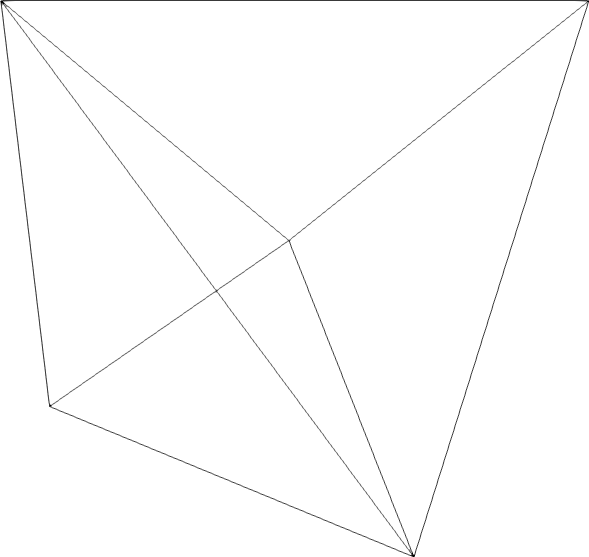
\includegraphics[height=3cm]{fig/1/5.png}
  \caption{Triangulation\_3}
  \label{fig:1-5}
\end{figure}
\begin{figure}[!htbp]
  \centering
  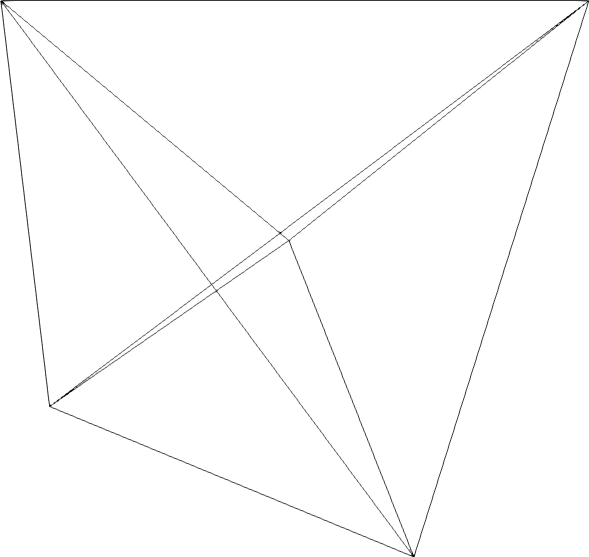
\includegraphics[height=3cm]{fig/1/6.png}
  \caption{Delaunay\_triangulation\_3}
  \label{fig:1-6}
\end{figure}
\begin{figure}[!htbp]
  \centering
  
\includegraphics[height=3cm]{fig/1/7.png}
  \caption{make\_mesh\_3}
  \label{fig:1-7}
\end{figure}


\subsection{Triangle}

Triangle是一个二维Delauany网格剖分的软件,是Jonathan Richard Shewchuk开发的。软件包括四个文件,triangle.h和triangle.c,可视化用的showme.c,以及一个c语言接口例子tricall.c。很有意思的是showme是直接基于x11开发的。其中triangle.c中有main函数定义,可以直接从triangle.c编译成可执行程序,但是需要注释掉TRILIBRARY的定义,也可以将triangle.c编译成链接库,然后tricall.c调用链接库,将tricall.c编译成可执行程序,或者将triangle.c和tricall.c放在一起编译成可执行程序。Triangle中给了一个例子,读取A.poly文件中数据进行网格剖分,结果会生成A.1.*的文件,然后用showme打开。在CMakeLists里将var设置成ON,将lib设置成OFF,是将triangle.c编译成可执行程序,将lib设置成ON,编译成动态链接库,var设置成OFF,是将triangle.c和tricall.c一起编译成可执行程序。运行install.sh文件,编译安装后在triangle$\_$install/bin文件夹中可以运行命令triangle$\_$run -p A进行测试,用命令showme A.poly打开查看。


\subsubsection{数据结构和算法}

Triangle里定义了网格数据结构mesh,mesh中定义了各种memorypool,其中包括vertices和triangles,memorypool是list中的一个节点,其中firstblock定义了初始位置,nowblock定义了当前位置,nextitem定义了下一个item位置,用poolalloc函数往memorypool里插入新节点,poolalloc会返回一个指针,指针类型可以是triangle、vertex等等,triangle是REAL类型的双重指针,可以对triangle进行赋值,vertex是REAL类型的指针,可以对vertex进行赋值。Triangle里定了命令行操作的数据结构behavior。Triangle网格剖分函数为delaunay,实现了三种剖分方法,分别为divconqdelaunay、incrementaldelaunay和sweeplinedelaunay函数,在incrementaldelaunay中insertvertex实现了Delaunay算法中的反转操作。

\subsubsection{算例}

\begin{figure}[!htbp]
  \centering
  
\includegraphics[height=3cm]{fig/1/8.png}
  \caption{Delaunay网格剖分发生翻转}
  \label{fig:1-7}
\end{figure}

\begin{figure}[!htbp]
  \centering
  
\includegraphics[height=3cm]{fig/1/9.png}
  \caption{在.poly中增加从$(1,0)$到$(0,1)$的约束,翻转不发生}
  \label{fig:1-7}
\end{figure}

\begin{figure}[!htbp]
  \centering
  
\includegraphics[height=3cm]{fig/1/10.png}
  \caption{用命令./trianglerun -pa0.001 A进行加密}
  \label{fig:1-7}
\end{figure}

\begin{figure}[!htbp]
  \centering
  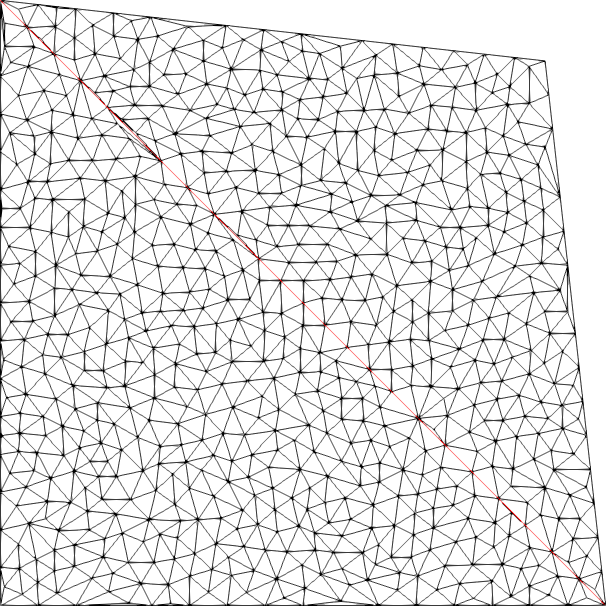
\includegraphics[height=3cm]{fig/1/11.png}
  \caption{在.poly中增加从$(1,0)$到$(0,1)$的约束,用命令./trianglerun -pa0.001 A进行加密}
  \label{fig:1-7}
\end{figure}

\begin{figure}[!htbp]
  \centering
  
\includegraphics[height=3cm]{fig/1/12.png}
  \caption{在.poly中增加从$(1,0)$到$(0,1)$的约束,用命令./trianglerun -pqa0.001 A进行加密和提高网格质量}
  \label{fig:1-7}
\end{figure}


\subsection{Tetgen}

Tetgen是德国Weierstrass Institute for Applied Analysis and Stochastics的Hang Si开发的,非常有意思的是Tetgen借鉴了很多triangle的工作,triangle是二维的Delaunay网格剖分,Tetgen是三维的Delaunay网格剖分,增加了网格自适应算法,Hang Si博士论文即为自适应算法。Tetgen并不复杂,主要包括tetgen.h和tetgen.cxx两个文件,可以用cmake生成Makefile并编译成可执行程序和链接库,需要在CMakeLists.txt中将BUILD$\_$EXECUTABLE或者BUILD$\_$LIBRARY设置成ON或者OFF,并且在tetgen.h中第55行修改TETLIBRARY定义。Tetgen读入的文件格式和triangle是一样的poly格式,poly格式是triangle开发者J. Shewchuk定义的,同样Tetgen采用了和triangle类似的命令行设置,Tetgen可以直接生成vtk格式的网格文件。

\subsubsection{数据结构和算法}
Tetgen包括tetgenio、tetgenbehavior、tetgenmesh,和triangle类似,其中tetgenio用于数据输入输出,tetgenbehavior用于操作设置,tetgenmesh是网格数据结构。网格数据结构中包括了REAL类型双重指针定义的tetrahedron和REAL类型指针定义的point,采用了triangle中的memorypool数据结构,定义了tetrahedrons和points,其外还定义了subfaces和subsegs。Delaunay网格剖分算法主要通过incrementaldelaunay函数和constraineddelaunay函数实现,incrementaldelaunay函数实现了两种算法,分别为the Bowyer-Watson (B-W) algorithm和the incremental flip algorithm of Edelsbrunner and Shah,incrementalflip函数实现反转功能。delaunayrefinement函数实现了网格加密,网格可以一致加密也可以局部加密。tetrahedralize函数是Tetgen网格剖分的接口。poly格式中定义顶点,首先定义顶点个数、空间维数、属性个数、标识个数,再具体定义。定义多面体面,首先定义面个数、标识个数,再定义每个面上多边形个数、孔个数、边界标识个数,再具体定义。

\subsubsection{算例}

\begin{figure}[!htbp]
  \centering
  
\includegraphics[height=3cm]{fig/1/13.png}
  \caption{采用./tetgen -pk A.poly命令,k生成vtk,产生了翻转。}
  \label{fig:1-7}
\end{figure}

\begin{figure}[!htbp]
  \centering
  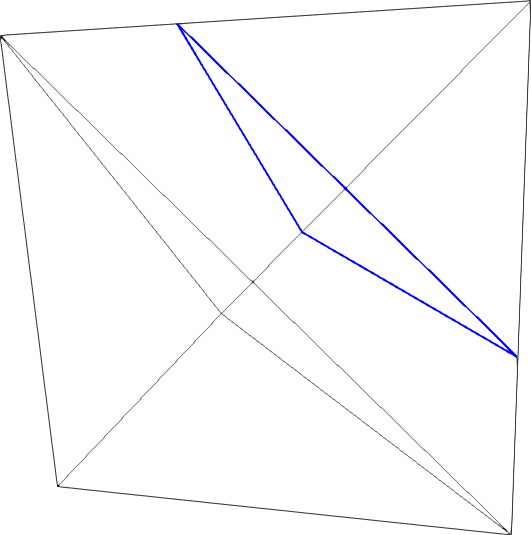
\includegraphics[height=3cm]{fig/1/14.png}
  \caption{采用./tetgen -pk A.poly命令,k生成vtk,将A.poly中12行注释掉,取消13行注释,27和28行取消注释,增加约束,抑制了翻转。}
  \label{fig:1-7}
\end{figure}

\begin{figure}[!htbp]
  \centering
  
\includegraphics[height=3cm]{fig/1/15.png}
  \caption{采用./tetgen -pka0.0001 A.poly命令,一致加密。}
  \label{fig:1-7}
\end{figure}

\begin{figure}[!htbp]
  \centering
  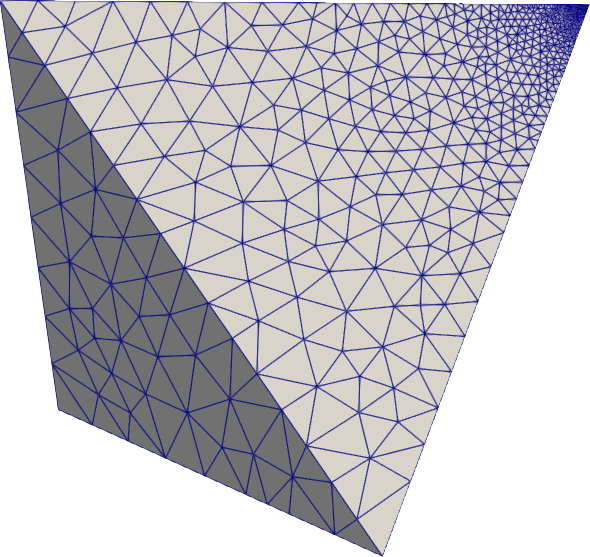
\includegraphics[height=3cm]{fig/1/16.png}
  \caption{采用./tetgen -pkqm A.poly命令,q提高网格质量并通过m读取A.mtr文件中间点密度条件。}
  \label{fig:1-7}
\end{figure}

\begin{figure}[!htbp]
  \centering
  
\includegraphics[height=3cm]{fig/1/19.png}
  \caption{采用./tetgen -pk example.poly命令。}
  \label{fig:1-7}
\end{figure}

\begin{figure}[!htbp]
  \centering
  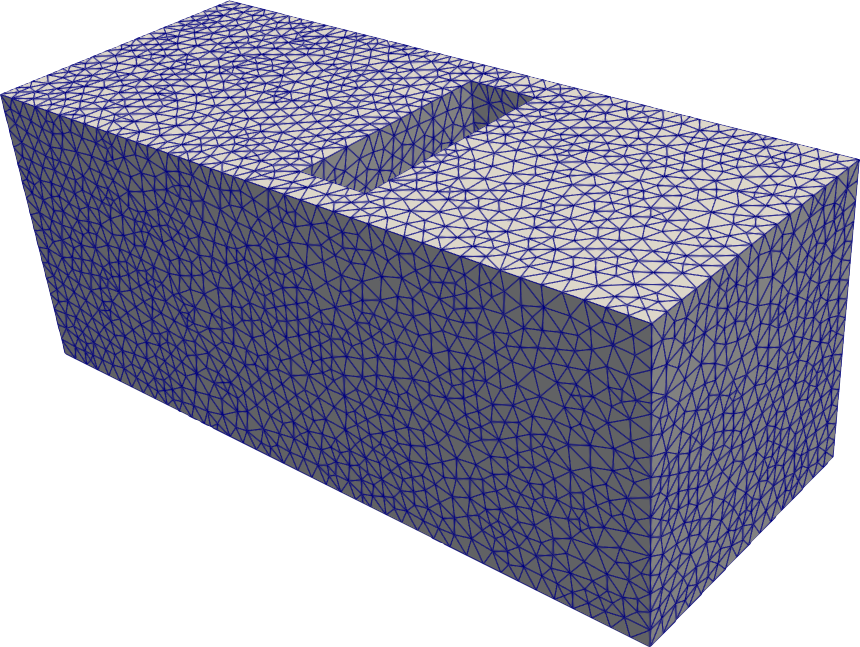
\includegraphics[height=3cm]{fig/1/17.png}
  \caption{采用./tetgen -pkqm example.poly命令。}
  \label{fig:1-7}
\end{figure}

\begin{figure}[!htbp]
  \centering
  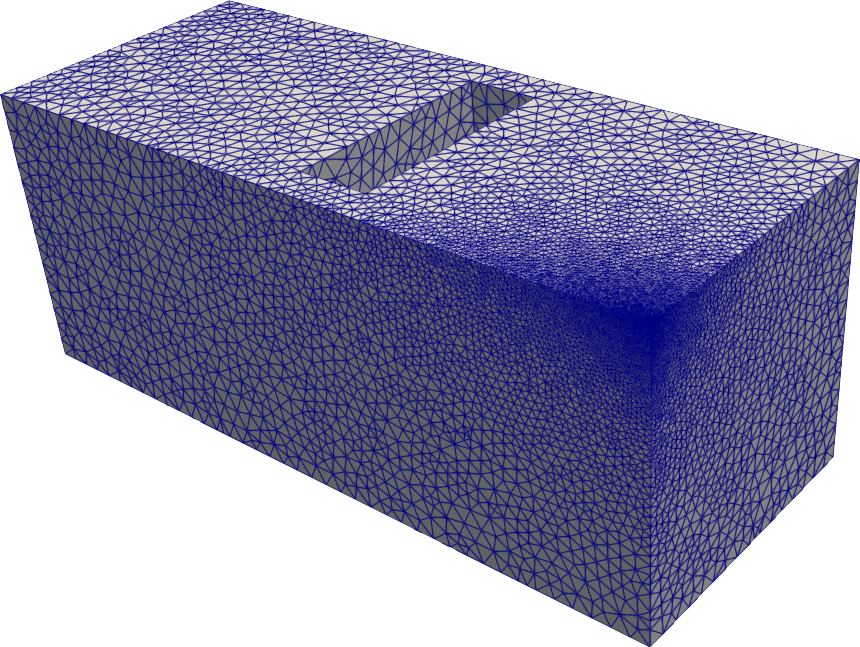
\includegraphics[height=3cm]{fig/1/18.png}
  \caption{采用./tetgen -pkqm example.poly命令,将第2行设置为0.001。}
  \label{fig:1-7}
\end{figure}


\subsection{Netgen}

Netgen的编译先去掉OCCT,因为OCE和OCCT版本不对。Netgen代码在libsrc路径下,编译后生成libngcore.so和libnglib.so两个链接库文件,再用cmake的find$\_$package调用Netgen的时候NETGEN$\_$LIBRARIES无效,需要指定链接库路径。Netgen安装在FENGSim/toolkit/install/netgen$\_$install,调用Netgen进行网格剖分的程序在FENGSim/starter/Mesh中,mkdir build/cd build/cmake ../make后,会生成mesh可执行程序在build中。
\subsubsection{数据结构和算法}
Netgen核心代码在libsrc路径下,接口代码在nglib路径下,见nglib.h。Netgen基本几何定义在libsrc/gprim路径下,几何点Point定义在libsrc/gprim/geomobjects.hpp中。Netgen网格剖分数据结构和算法都在libsrc/meshing路径下,其中libsrc/meshing/meshtype.hpp中定义了MeshPoint、Element,MeshPoint基于Point定义,网格数据结构定义在libsrc/meshing/meshclass.hpp中,其中T$\_$POINTS为网格顶点,基于MeshPoint定义的Array,之后还定义了segments、surfelements、volelements,volelements是基于Element定义的Array。FENGSim/starter/Mesh中的例子是对stl模型进行网格剖分,算法包括对边进行网格剖分,对面进行网格剖分,对实体进行网格剖分,分别调用了函数Ng$\_$STL$\_$MakeEdges、Ng$\_$STL$\_$GenerateSurfaceMesh、Ng$\_$GenerateVolumeMesh,这些函数都定义在FENGSim/toolkit/netgen/nglib/nglib.h中。Ng$\_$GenerateVolumeMesh函数中调用了MeshVolume函数,MeshVolume函数定义在FENGSim/toolkit/netgen/libsrc/meshing/meshfunc.hpp,MeshVolume函数中调用了MeshDomain函数,MeshDomain函数定义在FENGSim/toolkit/netgen/libsrc/meshing/meshfunc.hpp,MeshDomain中调用了unique$\_$ptr<Meshing3> meshing进行网格剖分,Meshing3类定义在FENGSim/toolkit/netgen/libsrc/meshing/meshing3.hpp中,实现了前沿推进法。前沿推进法可以和Delaunay进行混合,Netgen里还有单独的二维Delaunay网格剖分。

\subsubsection{算例}

\begin{figure}[!htbp]
  \centering
  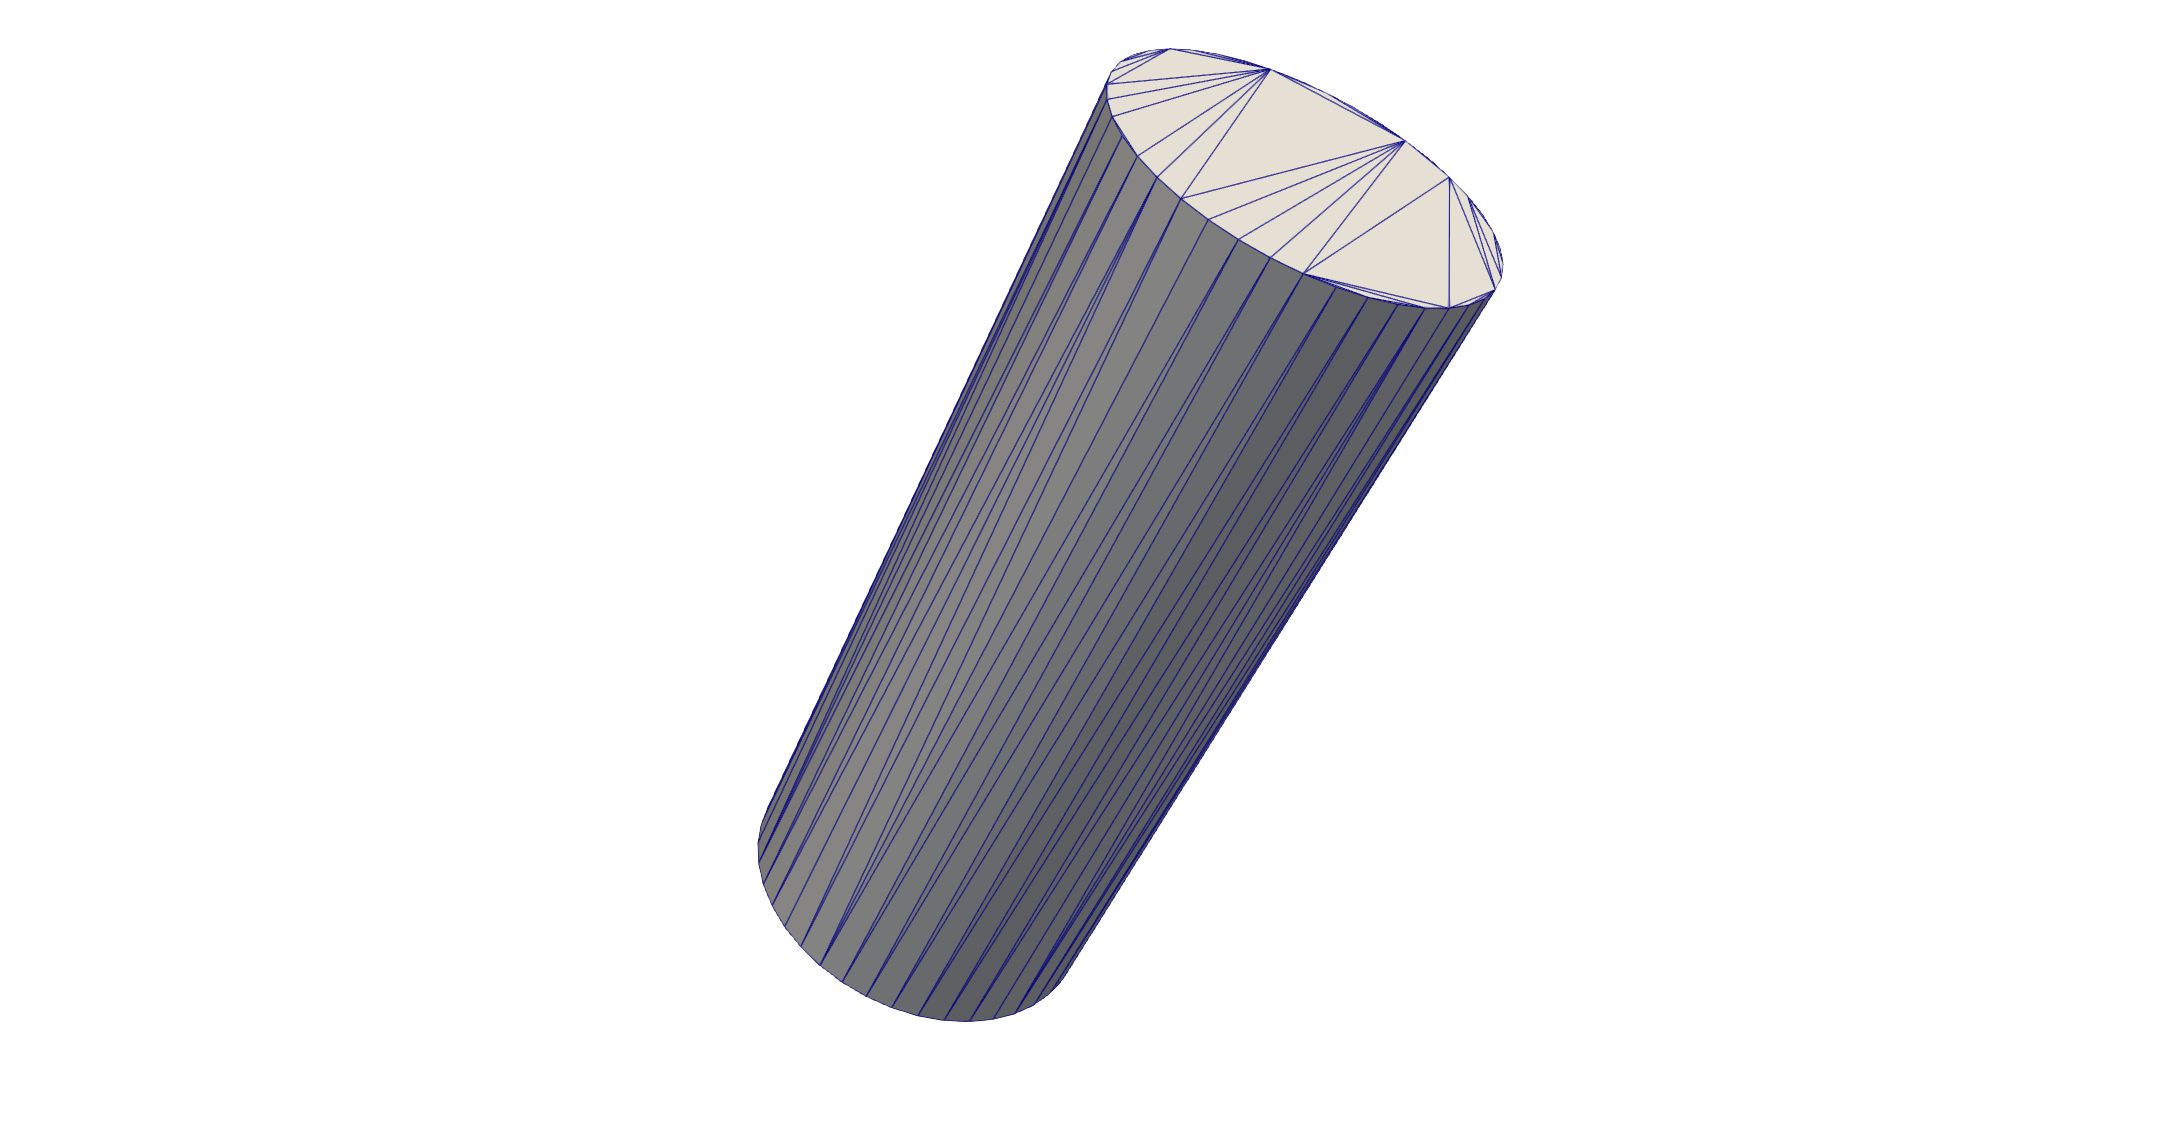
\includegraphics[height=3cm]{fig/1/1.1.4/1.png}
  \caption{./mesh ../data/2.stl,stl网格}
  \label{fig:1-7}
\end{figure}

\begin{figure}[!htbp]
  \centering
  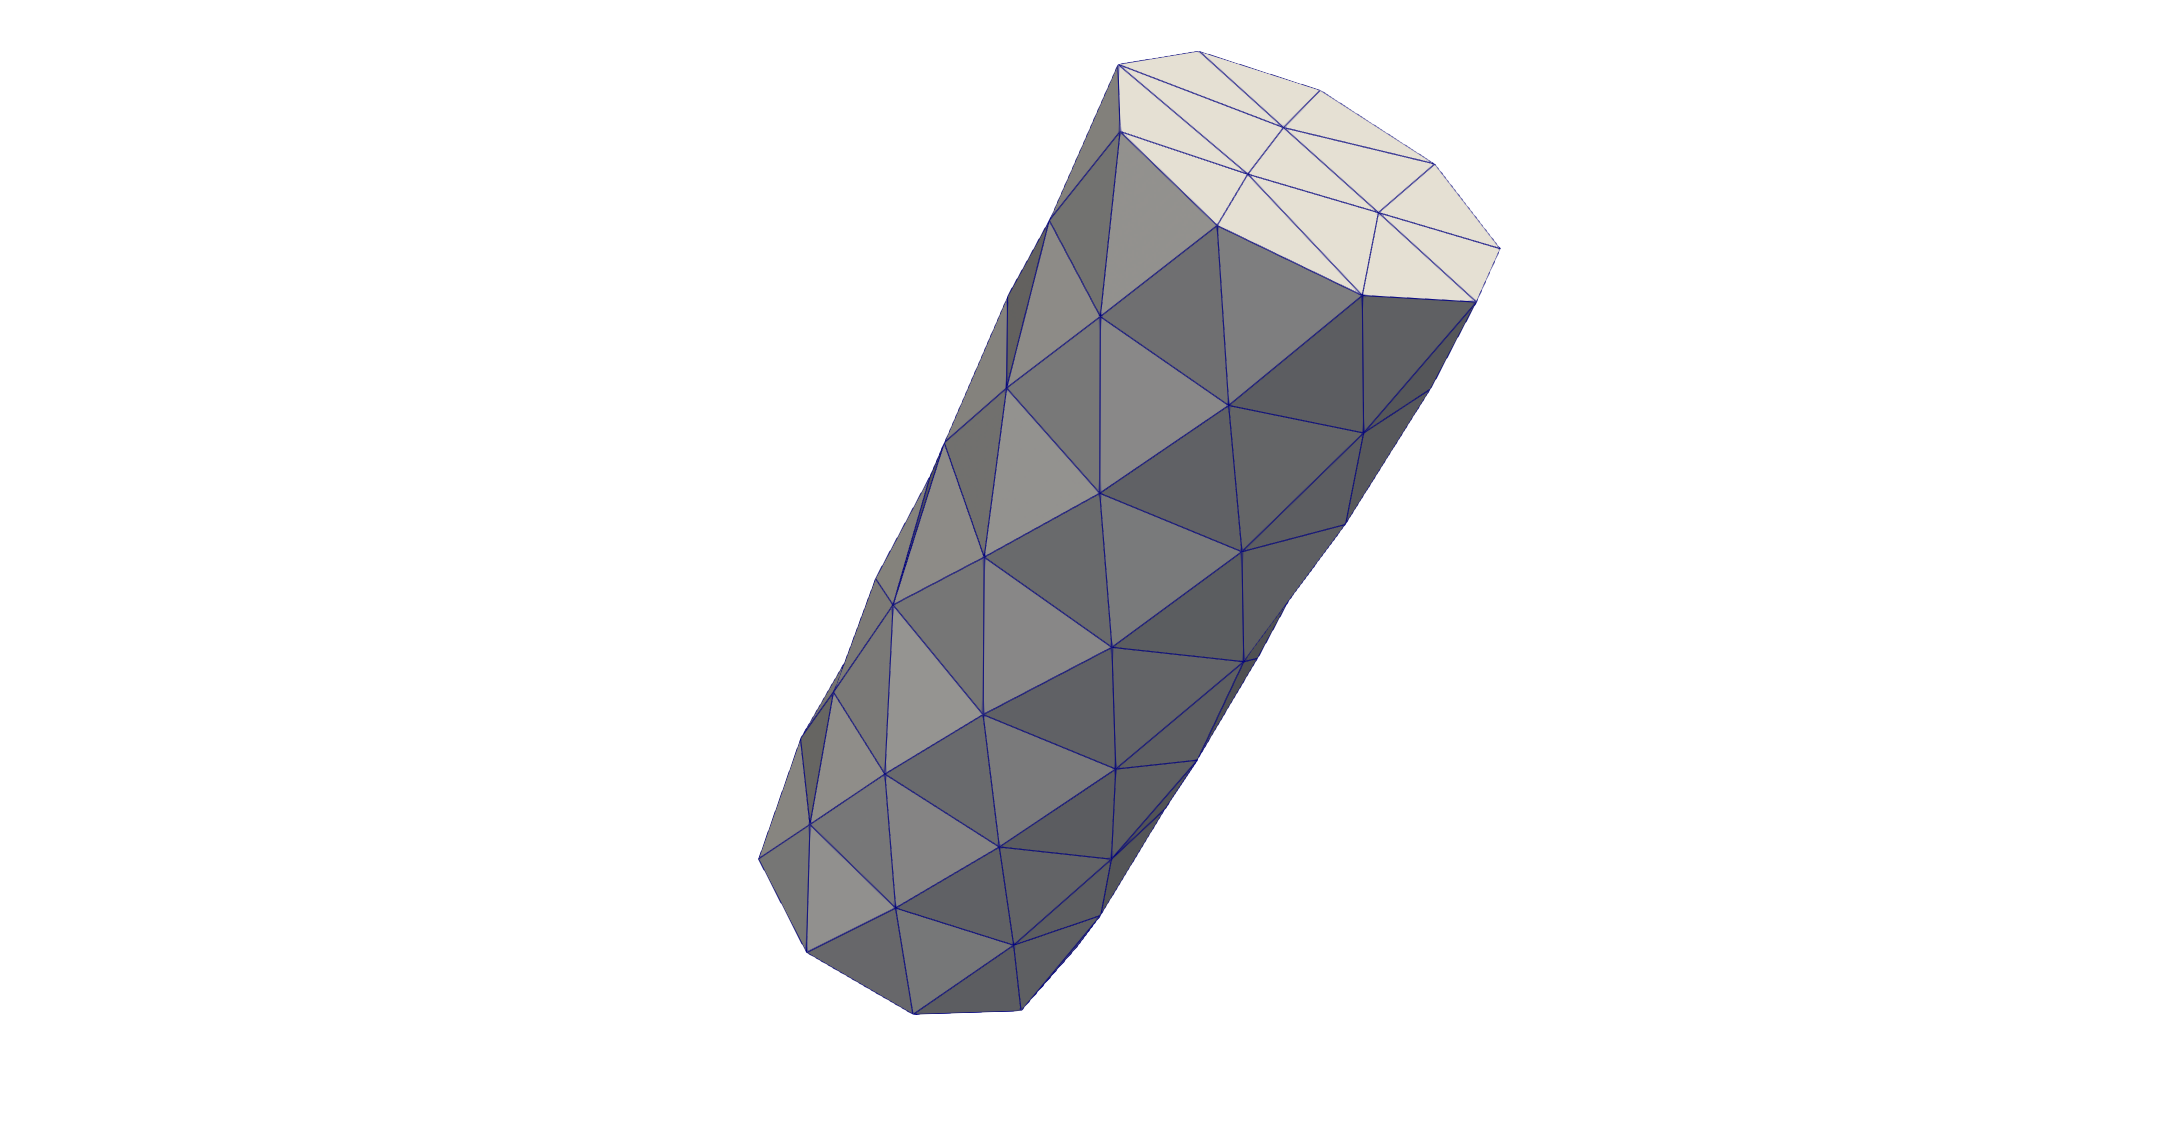
\includegraphics[height=3cm]{fig/1/1.1.4/2.png}
  \caption{./mesh ../data/2.stl,网格剖分}
  \label{fig:1-7}
\end{figure}

\begin{figure}[!htbp]
  \centering
  
\includegraphics[height=3cm]{fig/1/1.1.4/3.png}
  \caption{./mesh ../data/2.stl,网格加密}
  \label{fig:1-7}
\end{figure}

\begin{figure}[!htbp]
  \centering
  
\includegraphics[height=3cm]{fig/1/1.1.4/4.png}
  \caption{./mesh ../data/1.stl,stl网格}
  \label{fig:1-7}
\end{figure}

\begin{figure}[!htbp]
  \centering
  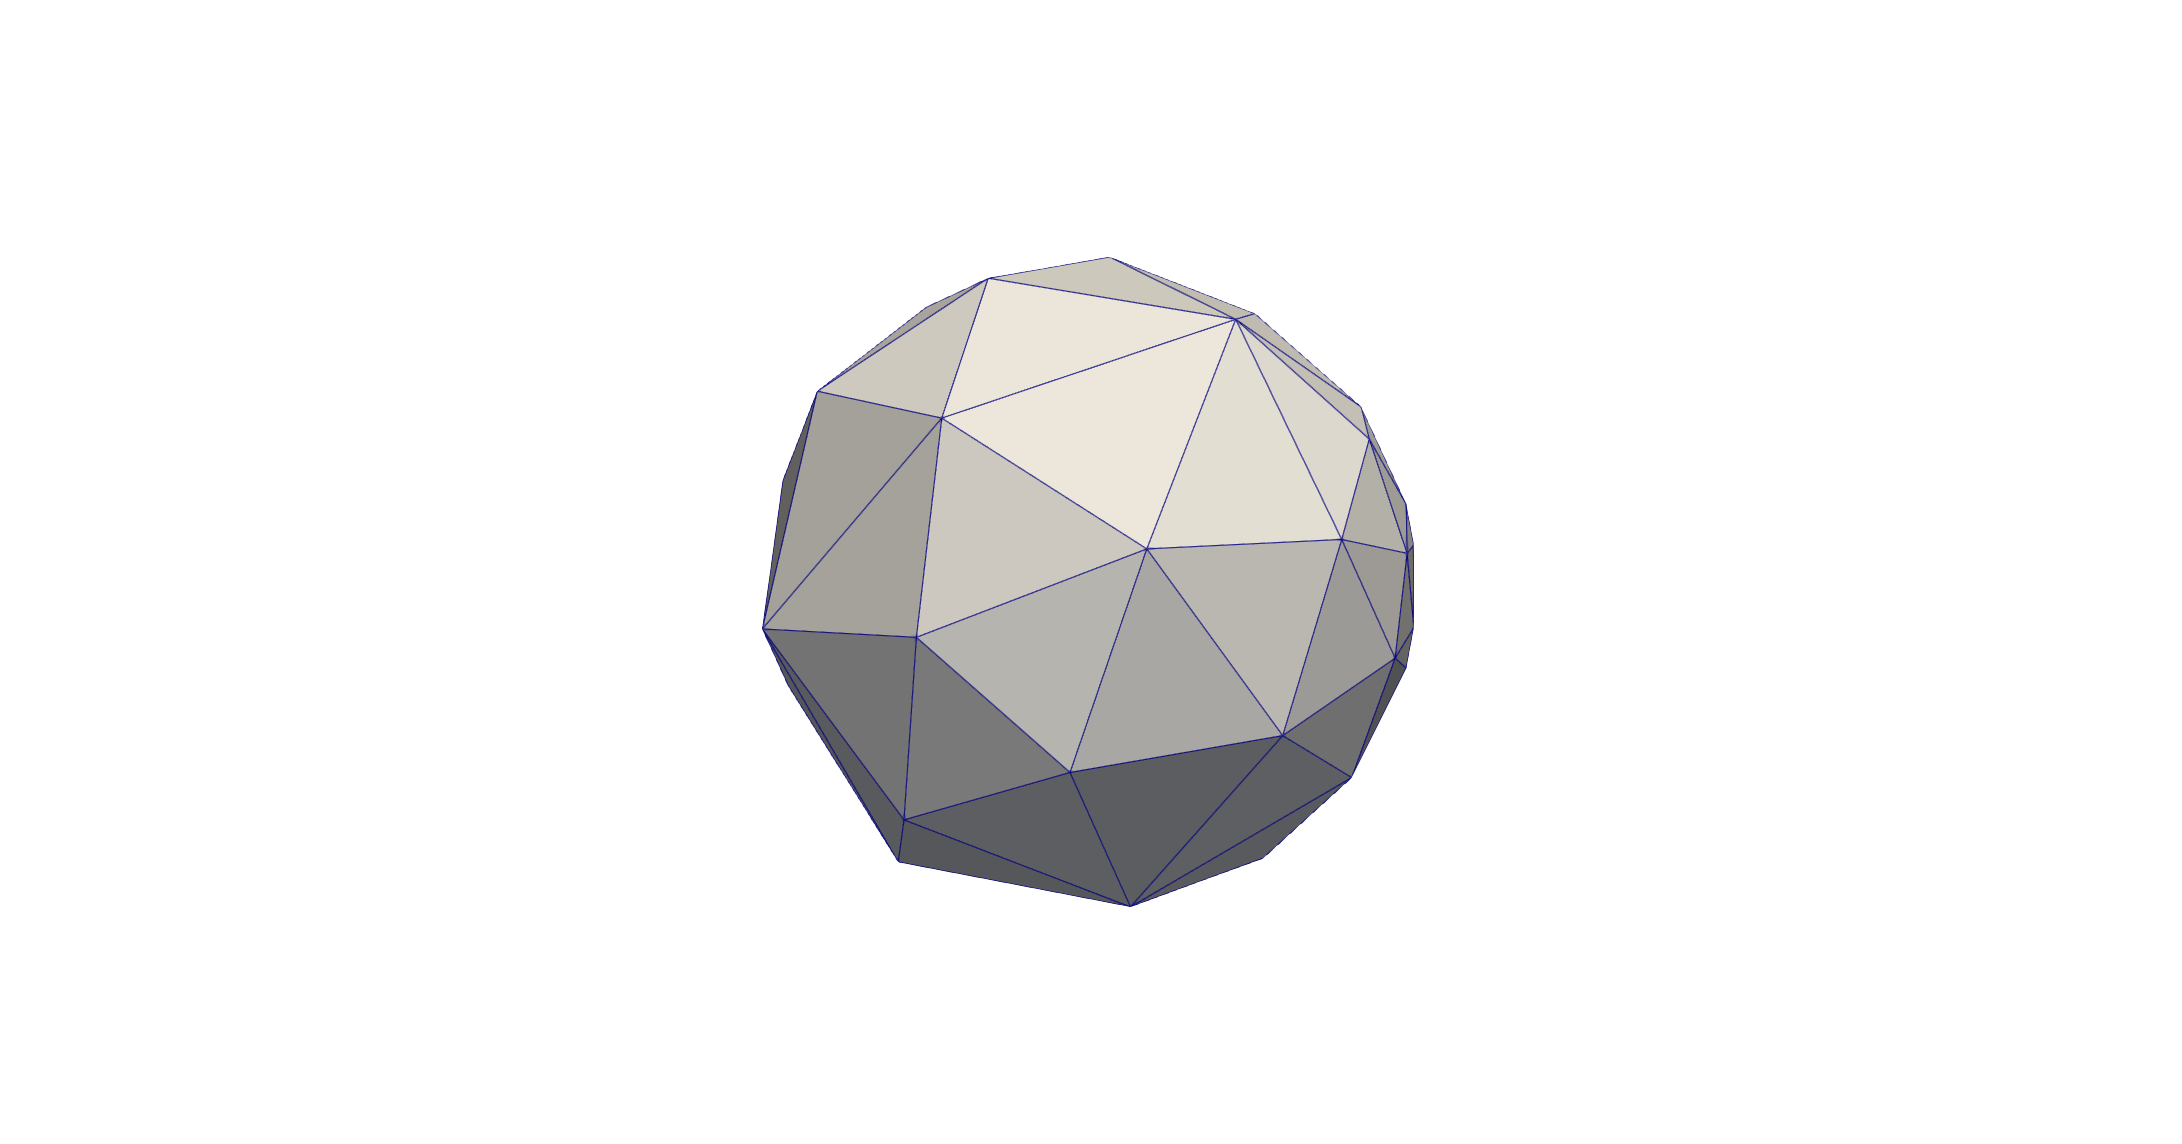
\includegraphics[height=3cm]{fig/1/1.1.4/5.png}
  \caption{./mesh ../data/1.stl,网格剖分}
  \label{fig:1-7}
\end{figure}

\begin{figure}[!htbp]
  \centering
  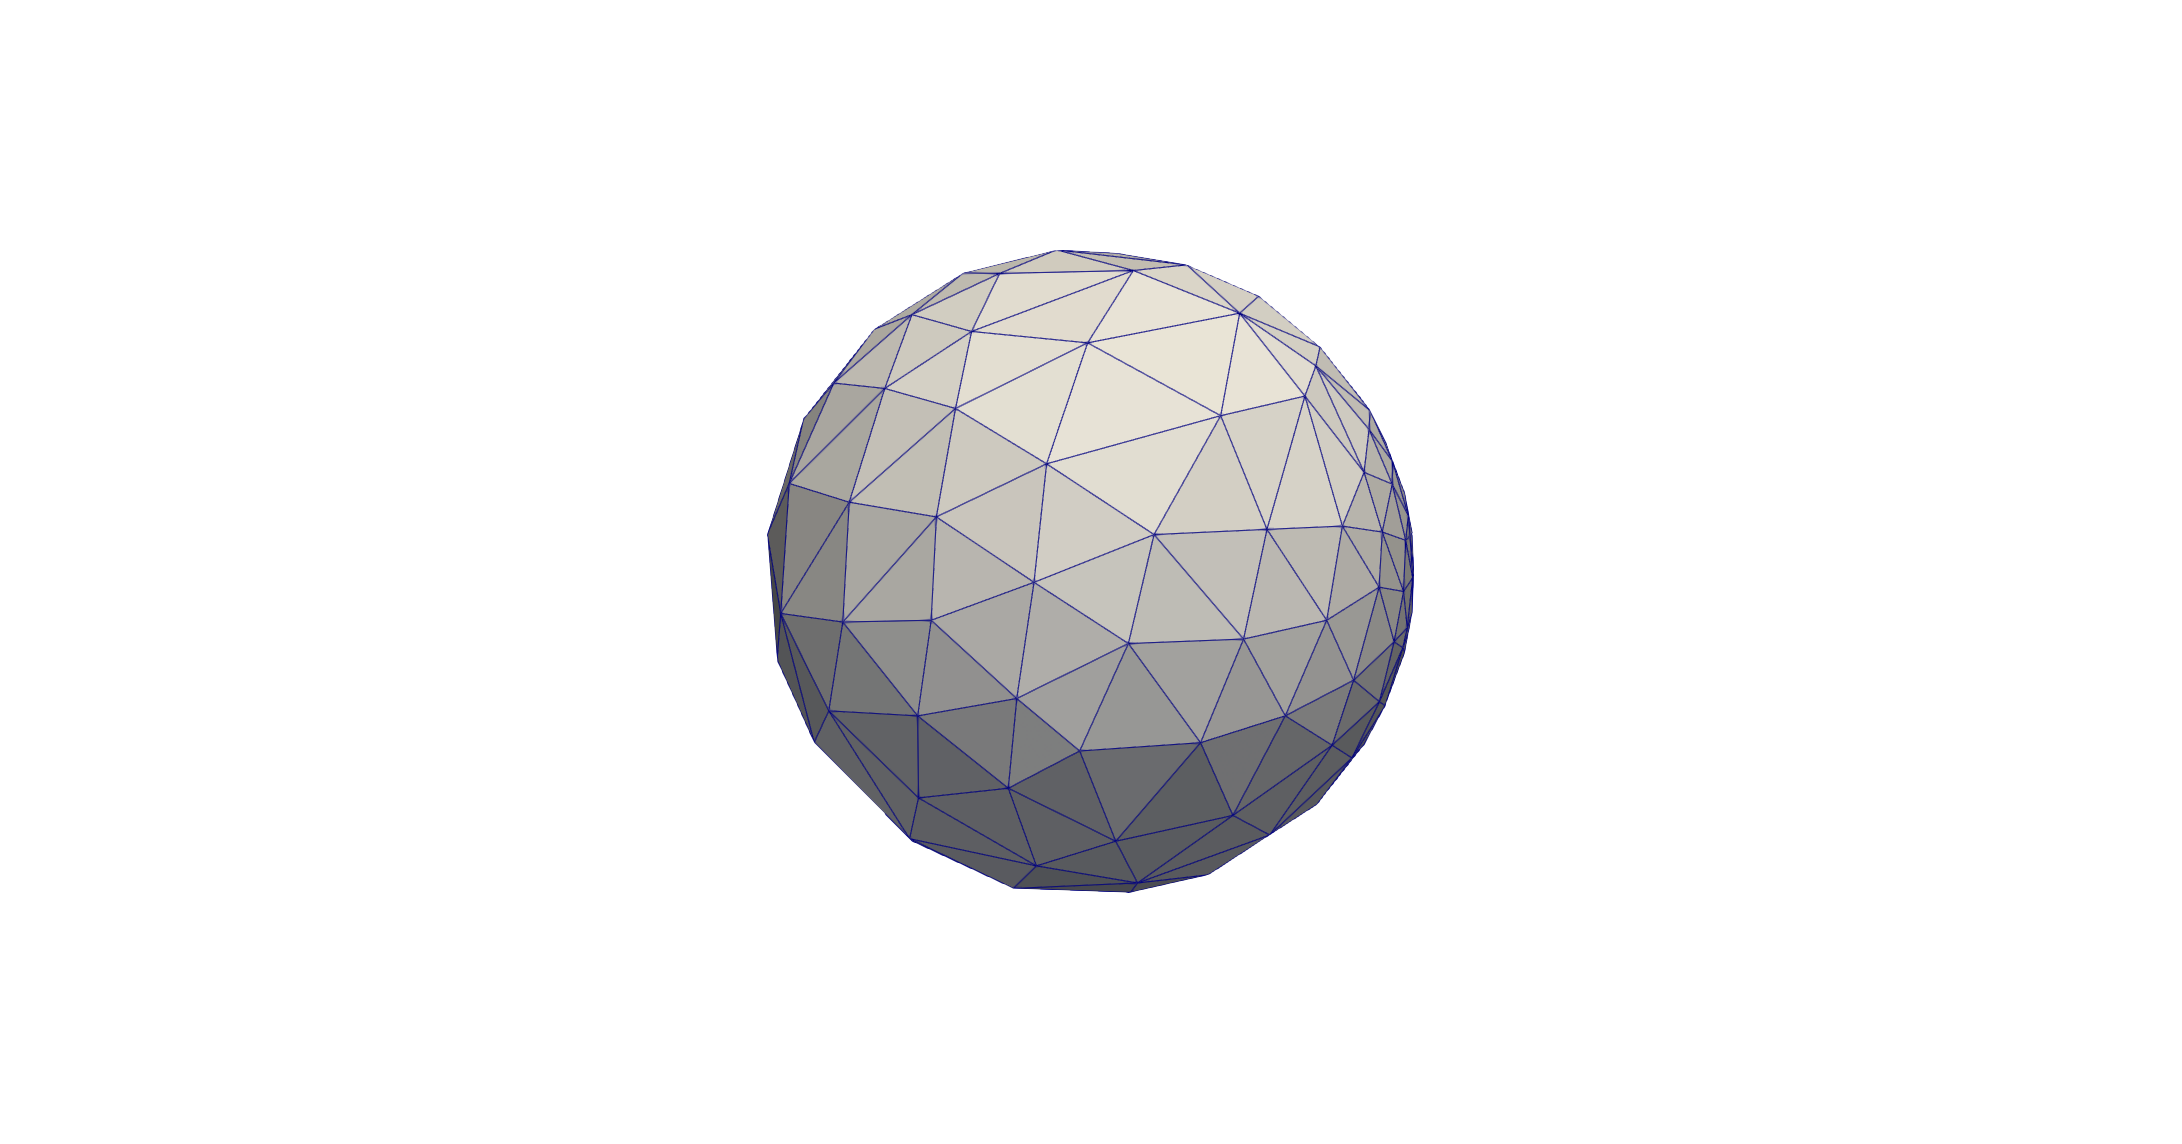
\includegraphics[height=3cm]{fig/1/1.1.4/6.png}
  \caption{./mesh ../data/1.stl,网格加密}
  \label{fig:1-7}
\end{figure}

\subsection{Gmsh}

\subsubsection{数据结构和算法}

\subsubsection{算例}

\subsection{Slice2Mesh}

Slice2Mesh是意大利CNR IMATI团队开发的,基于Triangle和Tetgen,Slice2Mesh原始是用Qt进行编译生成可执行程序,我们增加了CMakeLists进行编译。由于Slice2Mesh需要调用Triangle和Tetgen函数,需要将Triangle和Tetgen编译成链接库,编译链接库需要在triangle.c文件第236行定义TRILIBRARY,需要在tetgen.h文件第55行定义TETLIBRARY,实际上TRILIBRARY和TETLIBRARY定义是通过CMakeLists里的add$\_$definitions(CMakeLists第8行)和target$\_$compile$\_$definitions(CMakeLists第10行)定义的。编译后可在路径tool/install/triangle$\_$install和tool/install/tetgen$\_$install下找到相关头文件和动态链接库。slice2mesh还需要cinolib,cinolib只有头文件,不需要编译,cinolib也有cpp文件,但是只是被头文件引用。在slice2mesh引用cinolib头文件的时候,cinolib的CINOLIB$\_$USES$\_$BOOST、CINOLIB$\_$USES$\_$TRIANGLE、CINOLIB$\_$USES$\_$TETGEN需要在slice2mesh的CMakeLists中定义,建立cinolib和Boost、Triangle、Tetgen的接口,由于Tetgen头文件tetgen.h第2475行的tetrahedralize函数定义也需要TETLIBRARY定义,因此在slice2mesh引用Tetgen头文件的时候也需要定义TETLIBRARY,因此在slice2mesh的CMakeLists中第七行也定义了TETLIBRARY。

\subsubsection{数据结构和算法}

Slice2Mesh的算法分为三部分,首先对切片用Triangle进行二维网格剖分,然后将切片进行拉伸,进行网格协调性处理,再进行侧面网格剖分,最后生成Piecewise Linear Complex模型用Tetgen进行网格剖分,需要注意的是切片作为Tetgen的约束保证了层网格剖分。运行./slice2mesh$\_$exec ../data/pyramid$\_$l0.03.cli -tetflags a0.000001命令,然后运行python3 msh2vtk.py生成vtk文件。

Slice2Mesh中的Trimesh是来自cinolib,slice2plc将切片转为Piecewise Linear Complex模型,plc2tet进行内部网格剖分,在slice2plc中,先用mesh$\_$horizontal进行水平网格剖分,再用mesh$\_$vertical进行侧面网格剖分。Piecewise Linear Complex模型的三角单元都进行了标识,包括SRF$\_$FACE$\_$VERT、SRF$\_$FACE$\_$DOWN、SRF$\_$FACE$\_$U、PINTERNAL$\_$FACE,然后采用cinolib中的export$\_$cluster输出成off文件,off文件格式如下图。运行python3 plc2vtk.py可以将off文件转成vtk文件。读入文件格式为cli,COMMON LAYER INTERFACE,输出为mesh格式。

\begin{figure}[!htbp]
  \centering
  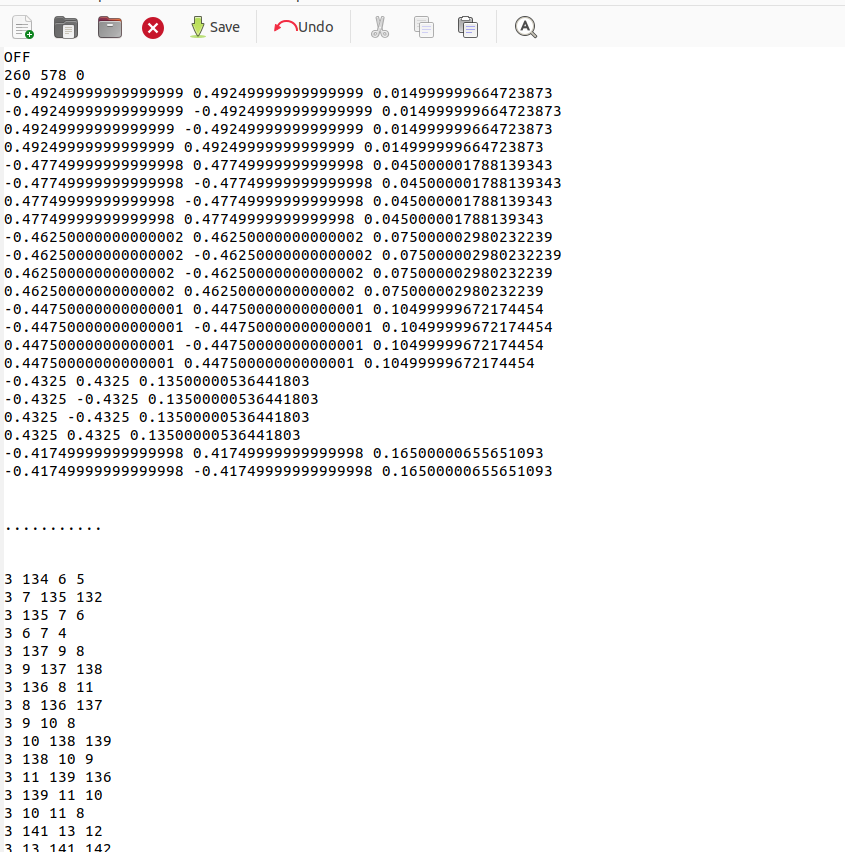
\includegraphics[height=5cm]{fig/1/1.1.7.1:0.png}
  \caption{off格式非常简单,图中260为定点个数,578为三角单元个数,定点坐标和单元编号之间没有其他注释。}
  \label{fig:1-7}
\end{figure}

\begin{figure}[!htbp]
  \centering
  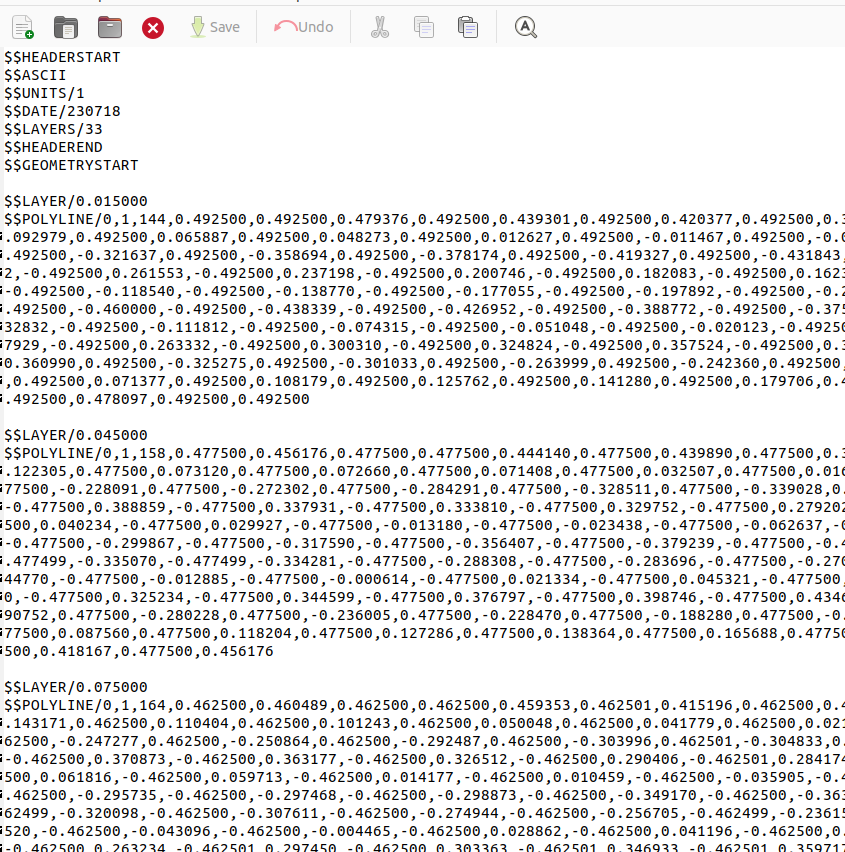
\includegraphics[height=5cm]{fig/1/1.1.7.1:00.png}
  \caption{cli格式非常简单,图中POLYLINE后边三位数,第一位为id,第二位为方向,可以是顺时针或者逆时针或者开放,第三位是该多边形顶点个数。}
  \label{fig:1-7}
\end{figure}

\begin{figure}[!htbp]
  \centering
  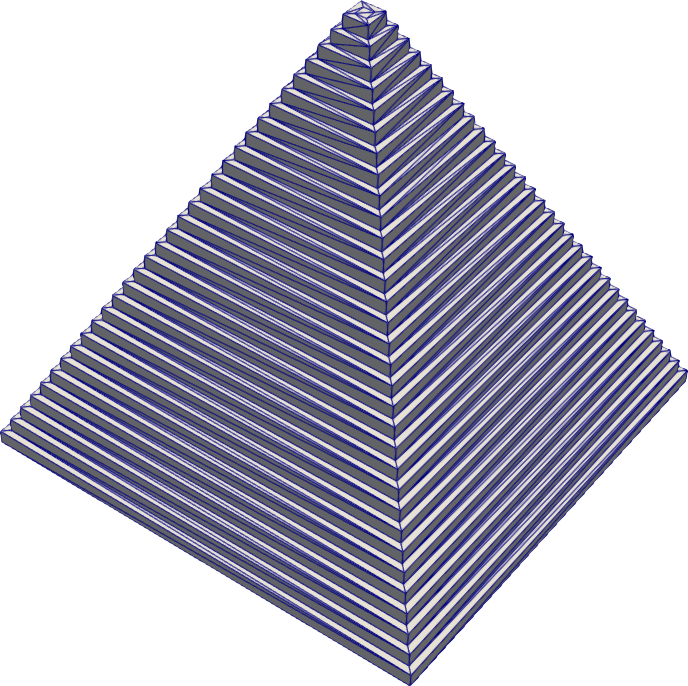
\includegraphics[height=3cm]{fig/1/1.1.7.1:1.png}
  \caption{采用./slice2mesh$\_$exec ../data/pyramid$\_$l0.03.cli命令生成amslices2mesh$\_$plc.off,修改plc2vtk.py中读入文件名称,用python3 plc2vtk.py生成vtk文件。}
  \label{fig:1-7}
\end{figure}

\begin{figure}[!htbp]
  \centering
  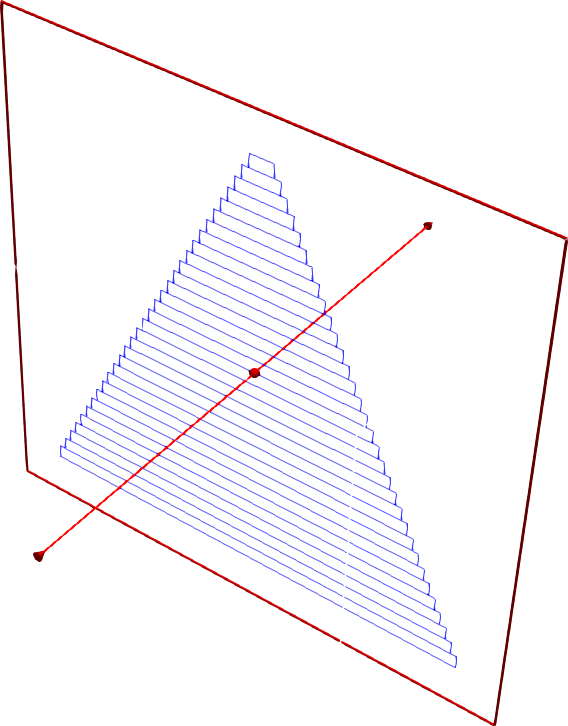
\includegraphics[height=3cm]{fig/1/1.1.7.1:2.png}
  \caption{采用./slice2mesh$\_$exec ../data/pyramid$\_$l0.03.cli命令生成amslices2mesh$\_$plc.off,修改plc2vtk.py中读入文件名称,用python3 plc2vtk.py生成vtk文件。}
  \label{fig:1-7}
\end{figure}

\begin{figure}[!htbp]
  \centering
  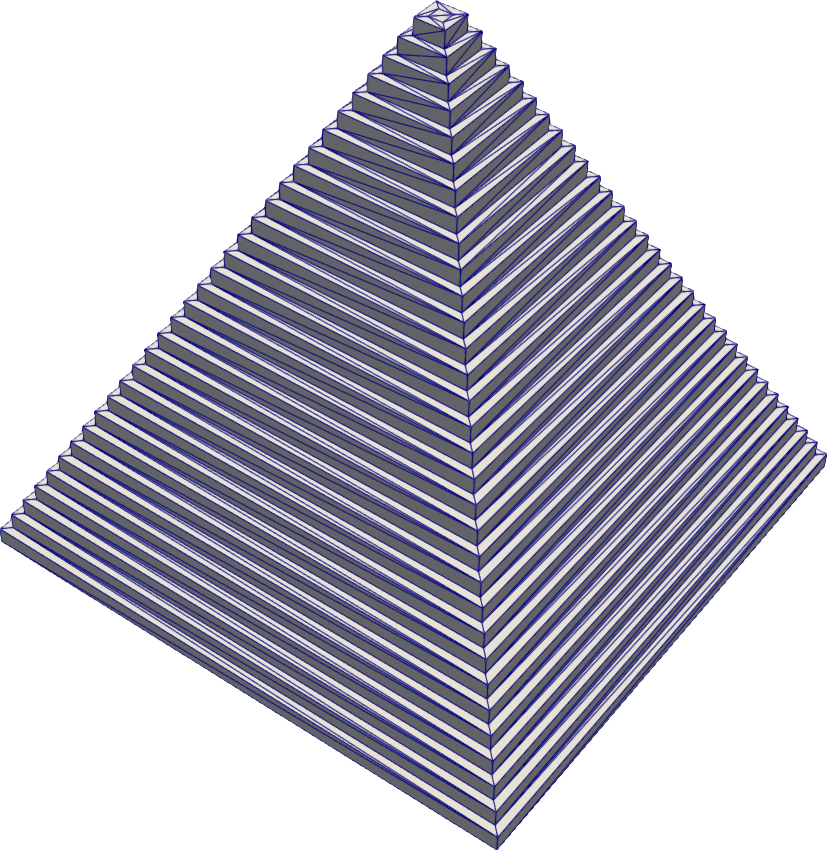
\includegraphics[height=3cm]{fig/1/1.1.7.1:3.png}
  \caption{采用./slice2mesh$\_$exec ../data/pyramid$\_$l0.03.cli命令生成amslices2mesh$\_$srf.off,修改plc2vtk.py中读入文件名称,用python3 plc2vtk.py生成vtk文件。}
  \label{fig:1-7}
\end{figure}

\begin{figure}[!htbp]
  \centering
  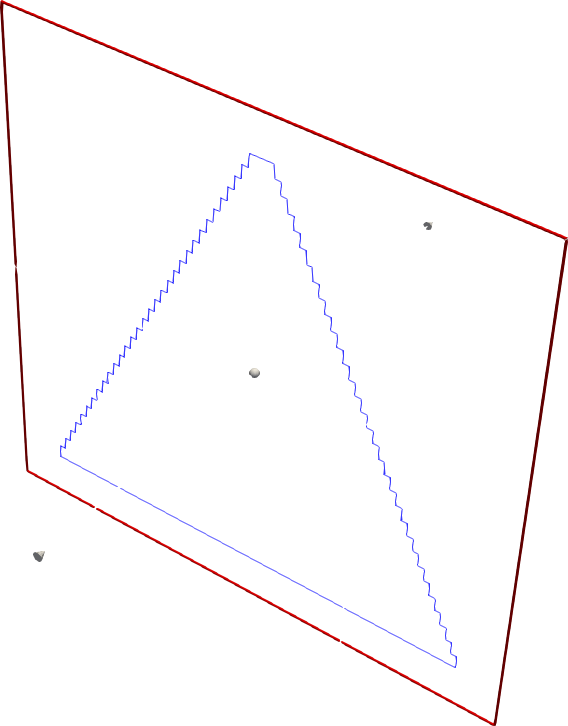
\includegraphics[height=3cm]{fig/1/1.1.7.1:4.png}
  \caption{采用./slice2mesh$\_$exec ../data/pyramid$\_$l0.03.cli命令生成amslices2mesh$\_$srf.off,修改plc2vtk.py中读入文件名称,用python3 plc2vtk.py生成vtk文件。}
  \label{fig:1-7}
\end{figure}

\begin{figure}[!htbp]
  \centering
  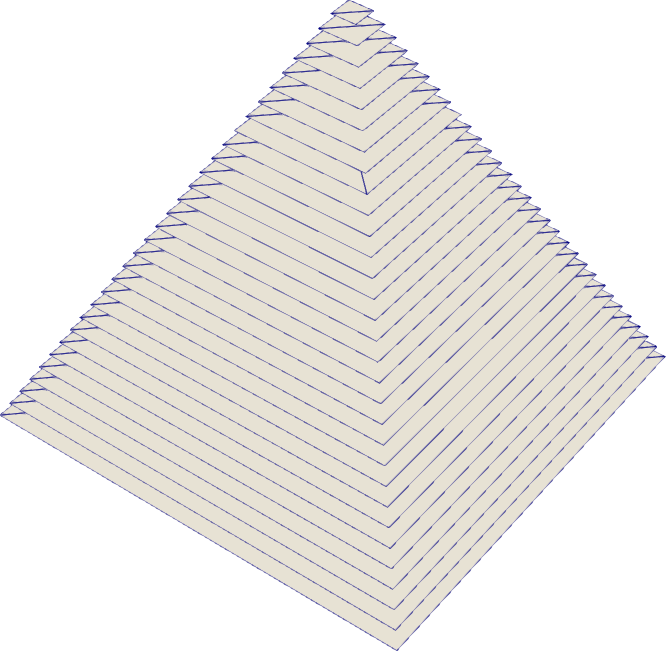
\includegraphics[height=3cm]{fig/1/1.1.7.1:5.png}
  \caption{采用./slice2mesh$\_$exec ../data/pyramid$\_$l0.03.cli命令生成amslices2mesh$\_$in.off,修改plc2vtk.py中读入文件名称,用python3 plc2vtk.py生成vtk文件。}
  \label{fig:1-7}
\end{figure}

\begin{figure}[!htbp]
  \centering
  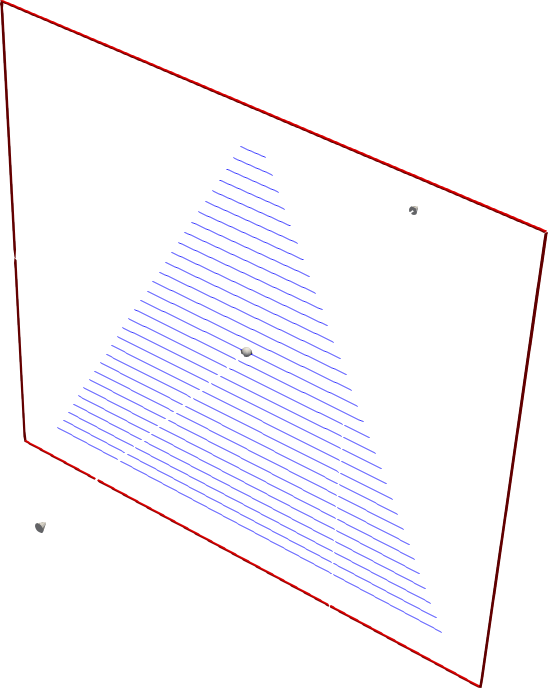
\includegraphics[height=3cm]{fig/1/1.1.7.1:6.png}
  \caption{采用./slice2mesh$\_$exec ../data/pyramid$\_$l0.03.cli命令生成amslices2mesh$\_$in.off,修改plc2vtk.py中读入文件名称,用python3 plc2vtk.py生成vtk文件。}
  \label{fig:1-7}
\end{figure}


\subsubsection{算例}

\begin{figure}[!htbp]
  \centering
  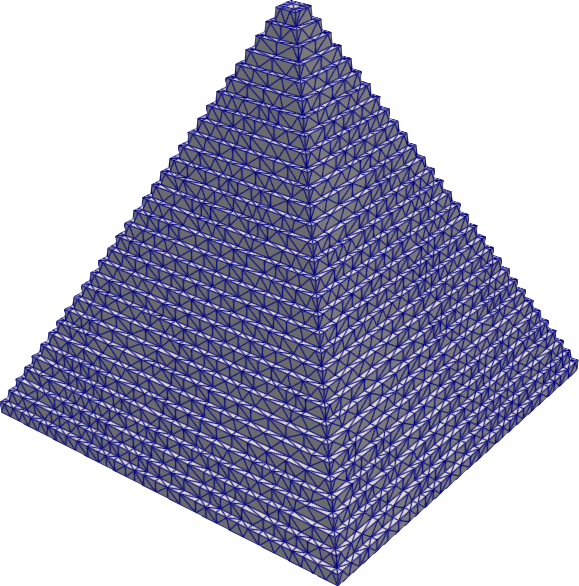
\includegraphics[height=3cm]{fig/1/20.png}
  \caption{采用./slice2mesh$\_$exec ../data/pyramid$\_$l0.03.cli -tetflags a1命令生成网格,用python3 msh2vtk.py生成vtk文件。}
  \label{fig:1-7}
\end{figure}

\begin{figure}[!htbp]
  \centering
  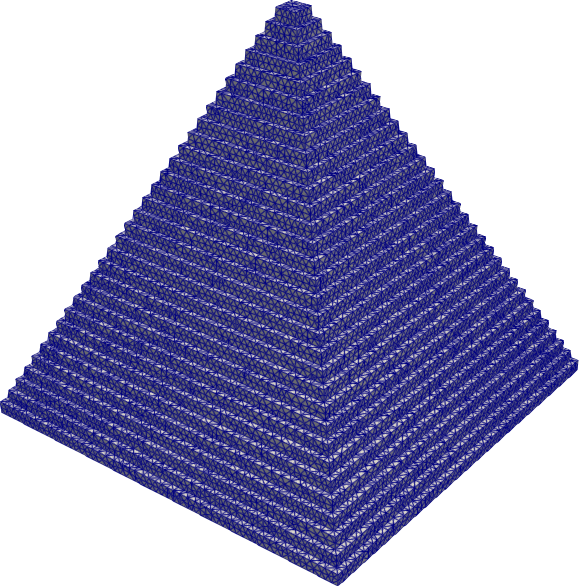
\includegraphics[height=3cm]{fig/1/21.png}
  \caption{采用./slice2mesh$\_$exec ../data/pyramid$\_$l0.03.cli -tetflags a0.000001命令生成网格,用python3 msh2vtk.py生成vtk文件。}
  \label{fig:1-7}
\end{figure}

\begin{figure}[!htbp]
  \centering
  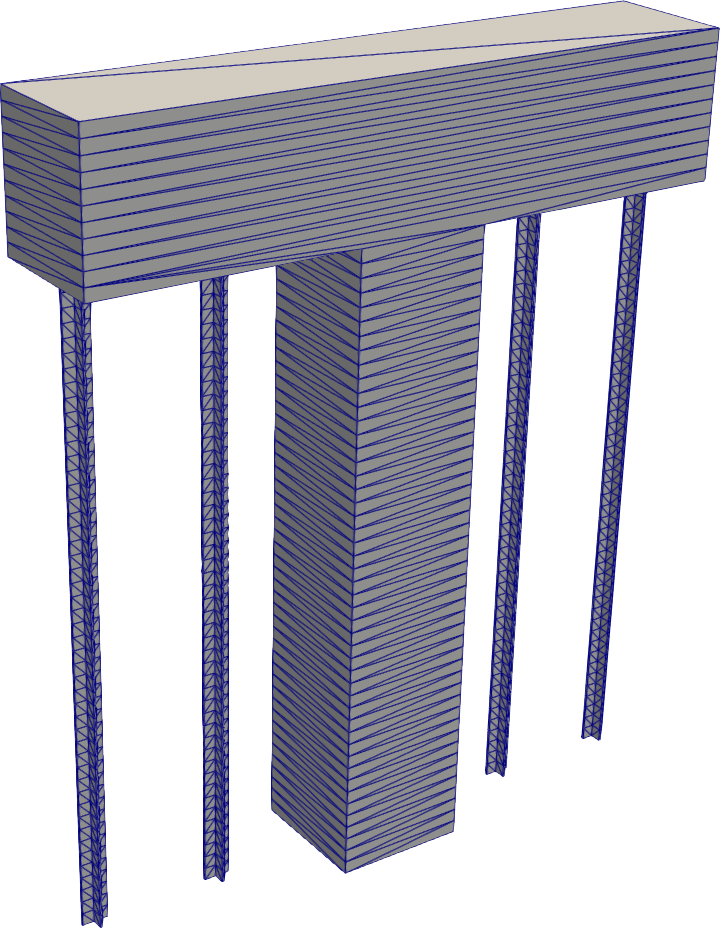
\includegraphics[height=3cm]{fig/1/1.1.7.2:3.png}
  \caption{采用./slice2mesh$\_$exec ../data/T$\_$supported.cli命令生成网格,用python3 msh2vtk.py生成vtk文件。}
  \label{fig:1-7}
\end{figure}

\begin{figure}[!htbp]
  \centering
  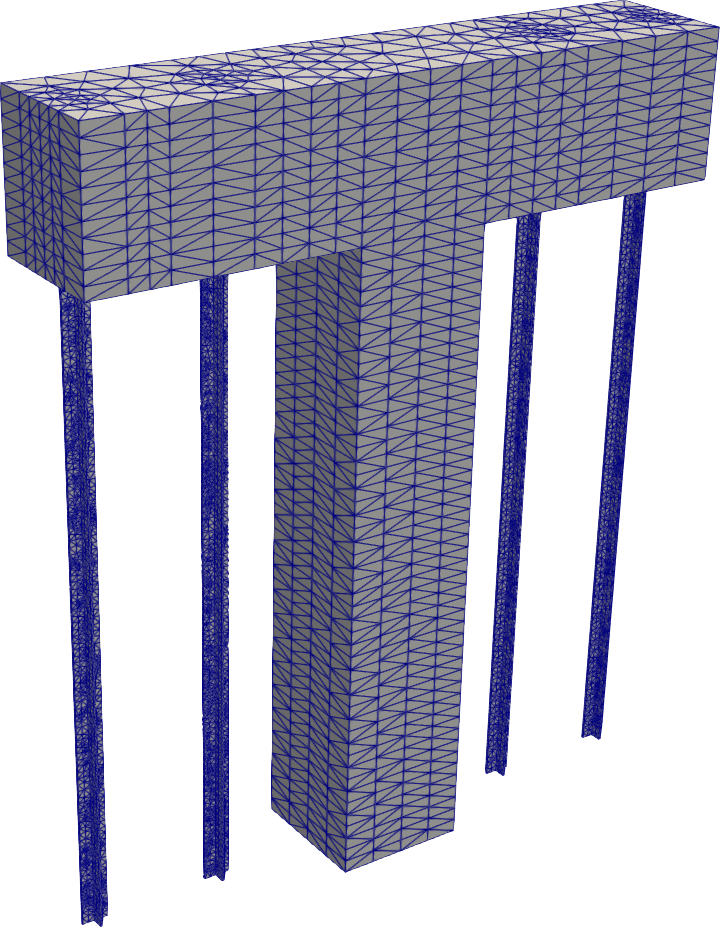
\includegraphics[height=3cm]{fig/1/1.1.7.2:4.png}
  \caption{采用./slice2mesh$\_$exec ../data/T$\_$supported.cli -tetflags a0.1命令生成网格,用python3 msh2vtk.py生成vtk文件。}
  \label{fig:1-7}
\end{figure}

\begin{figure}[!htbp]
  \centering
  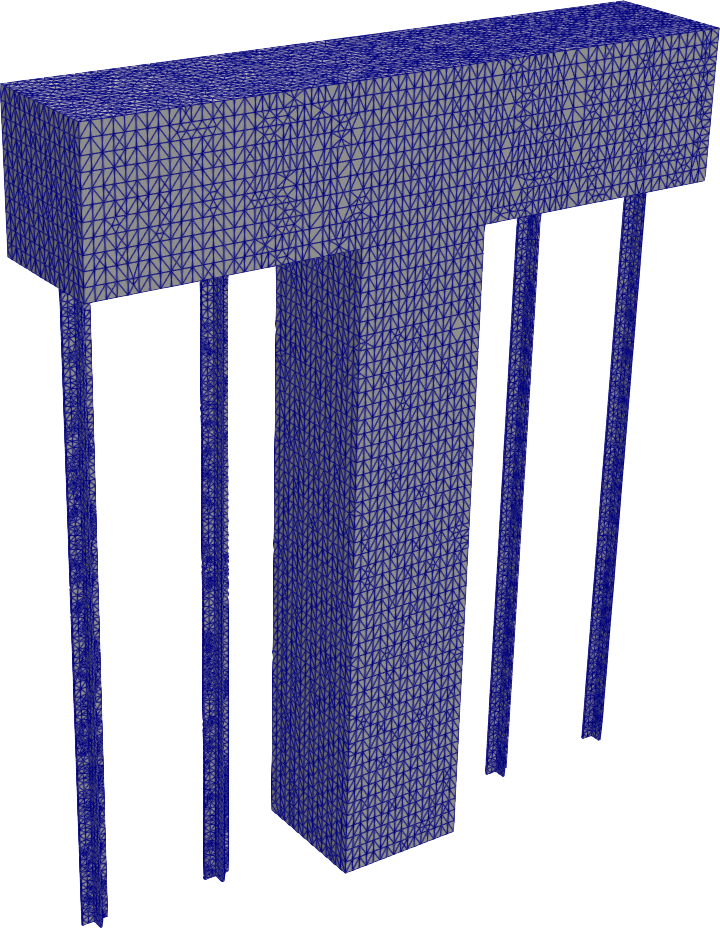
\includegraphics[height=3cm]{fig/1/1.1.7.2:5.png}
  \caption{采用./slice2mesh$\_$exec ../data/T$\_$supported.cli -tetflags a0.0001命令生成网格,用python3 msh2vtk.py生成vtk文件。}
  \label{fig:1-7}
\end{figure}


\section{结构性网格}

\subsection{RnD}

RnD是为了remapping开发的,首先是从四面体网格到六面体网格的remapping,需要四面体和六面体相交算法,然后计算moments,其中moments$\_$vox[0]为四面体和六面体相交的体积,因此除了做remapping,还可以对多面体进行像素网格剖分。将多面体进行四面体网格剖分,然后根据像素网格中六面体和四面体是否相交排除多余的六面体。在deprecated/examples/路径中有一个像素网格剖分的例子,其中vox$\_$size可以调整像素网格大小。

\subsubsection{数据结构和算法}
r3d$\_$dest$\_$grid为网格数据结构,定义在r3d.h中,定义四面体的面,用r3d$\_$voxelize$\_$tet函数计算像素网格和四面体相交,定义在r3d.h中,r3d$\_$dest$\_$grid的moments中保存了相交体积。

\subsubsection{算例}

\begin{figure}[!htbp]
  \centering
  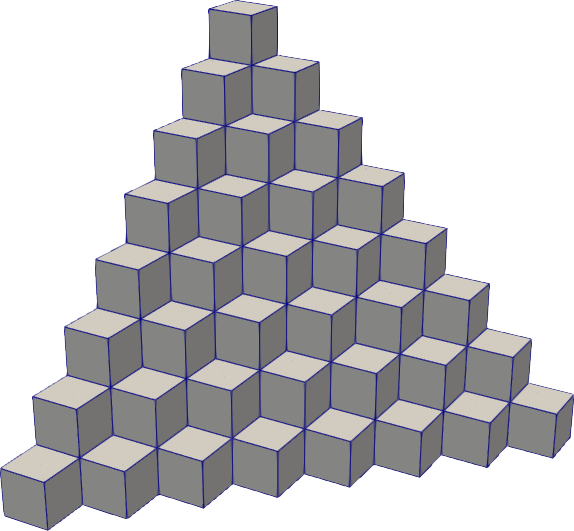
\includegraphics[height=3cm]{fig/1/1.2/1.png}
  \caption{$(0,0,0),(1,0,0),(0,1,0),(0,0,1)$,运行$.\\$voxelize,像素大小为$1/8$}
  \label{fig:1-7}
\end{figure}

\begin{figure}[!htbp]
  \centering
  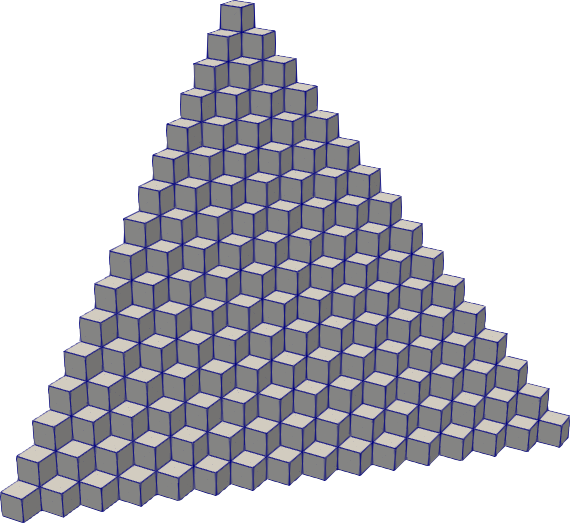
\includegraphics[height=3cm]{fig/1/1.2/2.png}
  \caption{$(0,0,0),(1,0,0),(0,1,0),(0,0,1)$,运行$.\\$voxelize,像素大小为$1/16$}
  \label{fig:1-7}
\end{figure}

\begin{figure}[!htbp]
  \centering
  
\includegraphics[height=3cm]{fig/1/1.2/3.png}
    \caption{$(0,0,0),(1,0,0),(0,1,0),(0,0,1)$,运行$.\\$voxelize,像素大小为$1/32$}
  \label{fig:1-7}
\end{figure}

\begin{figure}[!htbp]
  \centering
  
\includegraphics[height=3cm]{fig/1/1.2/4.png}
    \caption{$(0,0,0),(1,0,0),(0,1,0),(0,0,1)$,运行$.\\$voxelize,像素大小为$1/64$}
  \label{fig:1-7}
\end{figure}

\begin{figure}[!htbp]
  \centering
  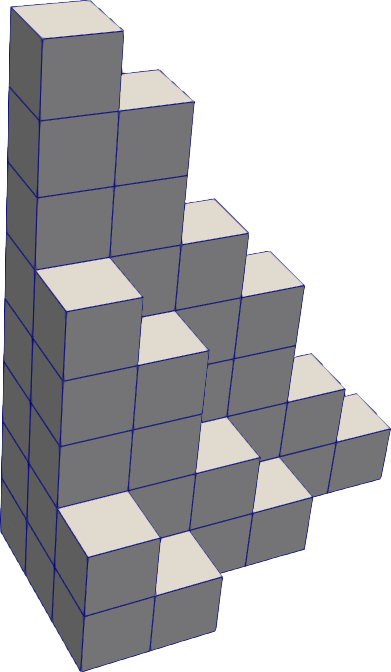
\includegraphics[height=3cm]{fig/1/1.2/5.png}
  \caption{$(0,0,0),(1/2,0,0),(0,1/3,0),(0,0,1/4)$,运行$.\\$voxelize,像素大小为$1/8$}
  \label{fig:1-7}
\end{figure}

\begin{figure}[!htbp]
  \centering
  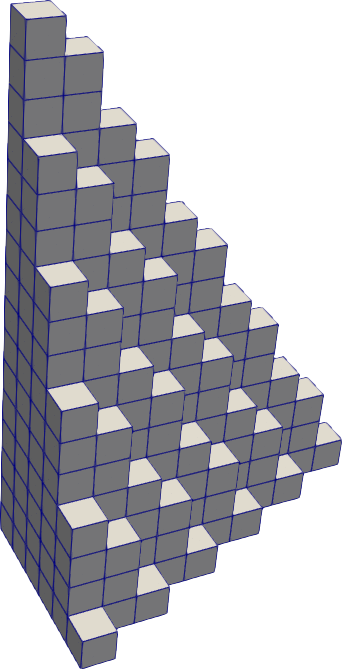
\includegraphics[height=3cm]{fig/1/1.2/6.png}
    \caption{$(0,0,0),(1/2,0,0),(0,1/3,0),(0,0,1/4)$,运行$.\\$voxelize,像素大小为$1/16$}
  \label{fig:1-7}
\end{figure}

\begin{figure}[!htbp]
  \centering
  
\includegraphics[height=3cm]{fig/1/1.2/7.png}
    \caption{$(0,0,0),(1/2,0,0),(0,1/3,0),(0,0,1/4)$,运行$.\\$voxelize,像素大小为$1/32$}
  \label{fig:1-7}
\end{figure}

\begin{figure}[!htbp]
  \centering
  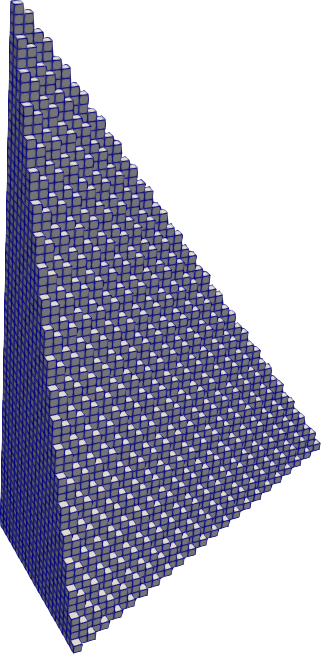
\includegraphics[height=3cm]{fig/1/1.2/8.png}
    \caption{$(0,0,0),(1/2,0,0),(0,1/3,0),(0,0,1/4)$,运行$.\\$voxelize,像素大小为$1/64$}
  \label{fig:1-7}
\end{figure}

\begin{figure}[!htbp]
  \centering
  
\includegraphics[height=3cm]{fig/1/1.2/9.png}
  \caption{$(0,0,0),(1,0,0),(0,1,0),(0,0,1),(0.9,0.9,0.9)$,运行$.\\$voxelize,像素大小为$1/8$}
  \label{fig:1-7}
\end{figure}

\begin{figure}[!htbp]
  \centering
  
\includegraphics[height=3cm]{fig/1/1.2/10.png}
    \caption{$(0,0,0),(1,0,0),(0,1,0),(0,0,1),(0.9,0.9,0.9)$,运行$.\\$voxelize,像素大小为$1/16$}
  \label{fig:1-7}
\end{figure}

\begin{figure}[!htbp]
  \centering
  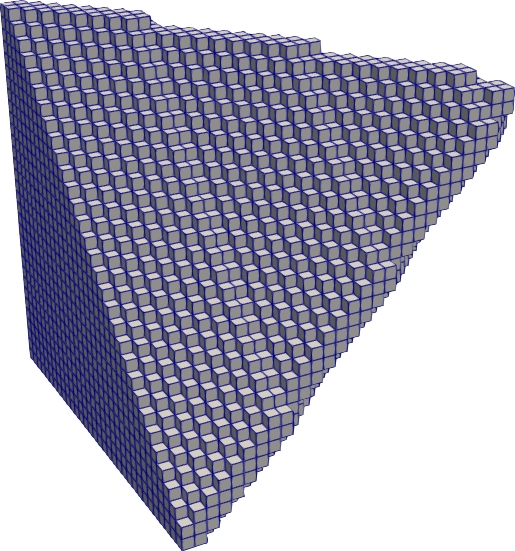
\includegraphics[height=3cm]{fig/1/1.2/11.png}
    \caption{$(0,0,0),(1,0,0),(0,1,0),(0,0,1),(0.9,0.9,0.9)$,运行$.\\$voxelize,像素大小为$1/32$}
  \label{fig:1-7}
\end{figure}

\begin{figure}[!htbp]
  \centering
  \includegraphics[height=3cm]{fig/1/1.2/12.png}
    \caption{$(0,0,0),(1,0,0),(0,1,0),(0,0,1),(0.9,0.9,0.9)$,运行$.\\$voxelize,像素大小为$1/64$}
  \label{fig:1-7}
\end{figure}

\newpage

对像素网格进行加密放粗,很容易获取非协调性网格,从而提高像素网格的模型精度,并降低网格数量。

\begin{figure}[!htbp]
  \centering
  \includegraphics[height=3cm]{fig/1/1.2/13.png}
  \caption{非协调性网格}
  \label{fig:1-7}
\end{figure}

\begin{figure}[!htbp]
  \centering
  \includegraphics[height=3cm]{fig/1/1.2/14.png}
  \caption{非协调性网格}
  \label{fig:1-7}
\end{figure}


\chapter{网格自适应性}

\section{网格自适应加密放粗}

网格自适应可以分为局部加密放粗和全局加密放粗,局部和全局的区别关键在于对初始网格的处理,局部网格剖分是对初始网格的修改,而全局网格剖分会重新生成新的网格。
局部加密放粗可以分为按顶点加密放粗和按单元加密放粗,全局加密放粗可以采用quadtree-octree(四叉树/八叉树)、advancing-front(前沿推进)和Delaunay类型的。
图\ref{fig:2-1}中用两个简单的例子说明按顶点加密放粗和按单元加密放粗,左上分图里红点为顶点,围绕该顶点有两条边,对两条边取中点得到两个新点,并和原有顶点相连,进行了细分,
左下分图里两个红点代表两个单元,将两个单元相邻边取中点,和边对面的顶点相连,分别将两个单元进行了细分得到了四个单元,并且保持协调性。全局加密放粗计算量大于局部,此外还有
hierarchic methods(继承方法)、多重网格、非协调和重叠方法,还需要考虑各向异性。

\begin{figure}[!htbp]
  \centering
  \includegraphics[height=5cm]{fig/2/1.png}
  \caption{按定点加密放粗和按单元加密放粗}
  \label{fig:2-1}
\end{figure}

以Tetgen为例测试局部加密放粗。第一个例子是通过插入点进行加密,第二个例子是通过设置单元大小进行加密,第三个例子是通过设置顶点网格密度进行加密。第一个例子通过.off格式文件读入
多面体,同时通过.node格式文件读入插入点,需要在操作命令序列中设置i命令。第二个例子需要读入网格文件,包括单元、面、边、点,同时通过.vol格式文件读入单元大小,需要注意的是操作命令序列中需要先设置r命令再设置a命令,设置r才会读入.vol文件,设置a会按照单元大小加密。第三个例子通过.poly格式文件读入多面体,同时通过.mtr格式文件读入顶点网格密度,需要在操作命令序列中设置m命令。

\begin{figure}[!htbp]
  \centering
  \includegraphics[height=3cm]{fig/2/2.png}
  \caption{例一:原始网格}
  \label{fig:2-1}
\end{figure}

\begin{figure}[!htbp]
  \centering
  \includegraphics[height=3cm]{fig/2/3.png}
  \caption{例一:插入1个点进行加密}
  \label{fig:2-1}
\end{figure}

\begin{figure}[!htbp]
  \centering
  \includegraphics[height=3cm]{fig/2/4.png}
  \caption{例一:插入7个点进行加密}
  \label{fig:2-1}
\end{figure}

\begin{figure}[!htbp]
  \centering
  \includegraphics[height=3cm]{fig/2/5.png}
  \caption{例一:原始网格一致加密后(pka0.001i),插入7个点再加密}
  \label{fig:2-1}
\end{figure}

\begin{figure}[!htbp]
  \centering
  \includegraphics[height=3cm]{fig/2/6.png}
  \caption{例一:原始网格一致加密后(pka0.001i),插入7个点再加密}
  \label{fig:2-1}
\end{figure}

\begin{figure}[!htbp]
  \centering
  \includegraphics[height=3cm]{fig/2/7.png}
  \caption{例二:原始网格,有三个单元}
  \label{fig:2-1}
\end{figure}

\begin{figure}[!htbp]
  \centering
  \includegraphics[height=3cm]{fig/2/8.png}
  \caption{例二:将第三个单元大小设置为0.1}
  \label{fig:2-1}
\end{figure}

\begin{figure}[!htbp]
  \centering
  \includegraphics[height=3cm]{fig/2/9.png}
  \caption{例二:将第三个单元大小设置为0.01}
  \label{fig:2-1}
\end{figure}

\begin{figure}[!htbp]
  \centering
  \includegraphics[height=3cm]{fig/2/10.png}
  \caption{例二:将第三个单元大小设置为0.001}
  \label{fig:2-1}
\end{figure}

\begin{figure}[!htbp]
  \centering
  \includegraphics[height=3cm]{fig/2/11.png}
  \caption{例二:将第三个单元大小设置为0.0001}
  \label{fig:2-1}
\end{figure}

\begin{figure}[!htbp]
  \centering
  \includegraphics[height=3cm]{fig/2/12.png}
  \caption{例三:原始网格,一共五个顶点}
  \label{fig:2-1}
\end{figure}

\begin{figure}[!htbp]
  \centering
  \includegraphics[height=3cm]{fig/2/13.png}
  \caption{例三:将所有顶点网格密度设置为0.25}
  \label{fig:2-1}
\end{figure}

\begin{figure}[!htbp]
  \centering
  \includegraphics[height=3cm]{fig/2/14.png}
  \caption{例三:将第一个顶点网格密度设置为0.05}
  \label{fig:2-1}
\end{figure}

\begin{figure}[!htbp]
  \centering
  \includegraphics[height=3cm]{fig/2/15.png}
  \caption{例三:将第一个顶点网格密度设置为0.01}
  \label{fig:2-1}
\end{figure}

\begin{figure}[!htbp]
  \centering
  \includegraphics[height=3cm]{fig/2/16.png}
  \caption{向指定位置插入点进行加密}
  \label{fig:2-1}
\end{figure}

\begin{figure}[!htbp]
  \centering
  \includegraphics[height=3cm]{fig/2/17.png}
  \caption{向指定位置插入点进行加密}
  \label{fig:2-1}
\end{figure}

\section{层网格自适应加密放粗}

\chapter{网格并行}

\section{M++}

\section{Metis}


\chapter{残余应力和变形}

\section{热弹塑性}

\section{小尺度热循环生死单元法}

\section{构件尺度固有应变法}


\clearpage

\bibliographystyle{plain}
\bibliography{sample}

\end{sloppypar}
\end{document}

